\documentclass[12pt,a4paper]{article}
\usepackage[latin1]{inputenc}
\usepackage{amsmath}
\usepackage{amsfonts}
\usepackage{amssymb}
\usepackage{hyperref}
\usepackage{parskip}
\usepackage{pgfplots}
\pgfplotsset{compat=1.16}
\usepackage[left=2cm,right=2cm,top=2cm,bottom=2cm]{geometry}
\author{Samuel Russell}
\title{Innocuous Ciphertexts}
\begin{document}
\maketitle

\section{Contributions}

\begin{itemize}
\item Critically discuss the downfalls of using an FTE system to encode ciphertexts.
\item Build a statistical tool for distinguishing emulated from normal traffic.
\item Build a new scheme that is able to overcome this detection.
\end{itemize}

\pagebreak
\section{Cryptography Background}
After language was invented to share knowledge, humans soon needed a way hide it from those whom it was not intended. The first schemes used word or letter substitutions or the shuffling of characters to make the meaning of a message hard to obtain. These techniques are still used as the basic building blocks today; for example in the AES block cipher, a very popular encryption scheme, of which there are hardware implementations baked in to many of the major computer chips. Early schemes however, relied on the secrecy of the method to protect the privacy of the message which meant that they cannot be reused by others. This lead to the introduction of parametrised constructions that use a key to alter the encryption such as the Vigen\`ere cipher. Modern schemes obey Keroff's principle; that the security of the system only depends on the security of the key, allowing the same encryption method to be used by all.
\begin{itemize}
 \item security through obscurity
 \item perfect security - information-theoretic
 \item conditional security
 \item ciphertexts - formatting
 \item block ciphers
\end{itemize}

\begin{itemize}
 \item hiding existence
 \item stenography
 \item honey encryption
 \item deniable encryption
\end{itemize}

\pagebreak
\section{Format Transforming Encryption}

In 1981, NIST\cite{FIPS74} outlined a mode of DES that was able to restrict the ciphertext of an encryption to a string of a fixed, finite alphabet such as decimal digits $ \Sigma = \{0,1...9\} $. This allows plain texts such as phone numbers of form $ X \in \Sigma^N $ to be encrypted to a ciphertext $ Y = \Sigma^N $ that is also a phone number. Although that FIPS document is now withdrawn it sparked further work such as Brightwell and Smith\cite{DPE}. They first specify the particular use case of encrypting data in place in a database where the ciphertexts must abide by the same type constraints of the database schema. The paper then goes on to describe their  Datatype-Preserving Encryption scheme that again works with DES in a streaming mode and works over an indexed finite alphabet, however the algorithm has redundant elements such as shuffling the alphabet's ordering that are not backed up with reasoning and there is no proof of security. More recently, Black and Rogaway\cite{CAFD} provide three constructions in their paper. They analyse the security of each one against the standard adversary $Adv^{prp}$ and also discuss the practical considerations of scaling.

The field has become a highly practical one, with companies such as Voltage moving to take advantage of the concept. They are using it to upgrade older systems by adding a layer of security that since does not change the structure of the data is invisible to the applications that sit on top. Therefore the costs of this retrofitting is vastly reduced since the need to completely redesign the system is usually eliminated. As of 2018, HPE\cite{hp} are still pushing it as part of their SecureData product to help maintain legacy software.

To keep up with the work in industry, Bellare et al. wrote a comprehensive paper\cite{fpe} that formally defines the goals of FTE. They did this in the form of adversary based games. They redefine the standard Pseudo Random Permutation (PRP) Security game which challenges an adversary to distinguish the encryption scheme from a random permutation. The paper also gives weaker notions they think are more appropriate. Single Point Indistinguishably (SPI) requires the adversary to be unable to distinguish between the encryption of any chosen plaintext and a randomly selected ciphertext. The Message Recovery (MR) game gives the adversary the distribution of plaintexts and asks for a decryption of a randomly selected ciphertext, given an encryption and verification oracle. Finally they define Message Privacy (MP) as the inability of an adversary to compute a function of a plaintext given the ciphertext; Note in this game the adversary can select the function it hopes it will have most success with. They state the following strength hierarchy for these games, showing PRP does give us the Message Recovery property we ultimately want.
$$ PRP \implies SPI \implies MP \implies MR $$
The first implication is trivial since a random function will produce a random element when given the message. The last last implications is also trivial since MR is just a special cast of MP - where the function is fixed to be the identity. For the proof of $ SPI \implies MP $ the paper shows how an adversary $B$ for SPI can be  constructed using an adversary $A$ for MP with sufficiently large advantage since $B$ is able to run $A$ and satisfy it's calls to the encryption oracle using its own oracle.
\subsection{Rank Then Encipher}
In the second half of the paper\cite{fpe} Bellare et al. then propose a framework called Rank then Encipher. This framework supports and enhances the methods already discussed since it enables any encryption scheme that supports arbitrary size alphabets to be used to encrypt more complex languages. It simplifies the complexity of language features such as a checksum character by maps words to an simple index so that the encryption scheme used can be generic. It does this by partitioning the language in to slices of the words of each length. That is, for the language $\mathcal{X} = \{\mathcal{X}_N : N \in \mathcal{N} \}$ for lengths $\mathcal{N}$, each slice $\mathcal{X}_N = \{ X : X \in \mathcal{X}, \vert X \vert = N  \}$. Now each slice can be arbitrarily ordered as $\mathcal{X} = \{ X_0, X_1, \cdots , X_{n-1} \} $ and a bijective mapping can be defined $rank_N :: \mathcal{X}_N \rightarrow \mathbb{Z}_n$.
Then for the whole language, we can define
$$ rank :: \mathcal{N} \times \mathcal{X} \rightarrow \mathbb{N} \cup \bot $$
$$ rank(N,X) =
\left\{
	\begin{array}{ll}
		rank_N(X)  & \mbox{if } \vert X \vert = N\\
		\bot & \mbox{otherwise} 
	\end{array}
\right.
$$

$$ unrank :: \mathcal{N} \times \mathbb{N} \rightarrow \mathcal{X} \cup \bot $$
$$ unrank(N,i) =
\left\{
	\begin{array}{ll}
		rank_N^{-1}(i)  & \mbox{if } i \in \mathbb{Z}_{\mathcal{X}_N}\\
		\bot & \mbox{otherwise} 
	\end{array}
\right.
$$\\\\
Then if we have an encryption scheme $Enc :: \mathcal{K} \times \mathcal{N} \times \mathbb{N} \rightarrow \mathbb{N}$ that works over arbitrary domains to encrypt values into $\mathbb{Z}_{|\mathcal{X}_N|}$, we can define out scheme $\mathcal{E}_k^N = unrank_N \cdot Enc_k^{|X_N|} \cdot rank_N$. Using this construction, they state how the security properties of the original encryption scheme over the finite domain is inherited by the the rank then encrypt scheme over the language.

They provide a ranking and un-ranking algorithm for regular languages, but to make this efficient, pre-computation is needed. For each word length a table has to be created which can be done through dynamic programming.

Furthermore, using M\"akinen's\cite{rankcf}, algorithms if a language can be described an unambiguous context free grammar then ranking can be done in linear time and unranking can be done in $O(n \log n)$ time, if we allow $O(n^2)$ time and space preprocessing. This is since the left Szilard language of the grammar can be more easily ranked and unranked. Conversion back to the original grammar is as simple as linearly applying the rules and conversion from a word to it's left Szilard counterpart depends on the efficiency of parsing, which, is not linear, but for unambiguous grammars is still efficient.

\begin{itemize}
 \item rank then encipher approach
 \item security notations
 \item application for proxy transport
 \item downfall
 \item opaque vs innocuous
\end{itemize}

\pagebreak
\section{Motivation}

Tim Berners-Lee says\cite{gard} that since its conception, the world wide web has been built with the principles of openness and privacy. These key values, that also lie at the heart of democracy, can ensure that if a website is made available on web, anyone can connect to it - no matter who they are or where they live. 

However, recently, changes have been made which challenge this status quo. These changes are the censorship of certain content on the internet for users in some places like the United Kingdom or in China. The motivations behind this censorship can be well-meaning, for example, the blocking of illegal content such as child pornography with the intention of protecting the innocent lives of children. Further attempts to reduce damage to people's lives was the implementation of search engine de-listing of personal content partitioned by the right-to-be-forgotten movement\cite{rtbf}. This decision sparked much controversy since people believed that this deletion of history could lower the quality of the internet. 

However, other cases are on a much larger scale, such as nation states blocking access to content that they deem to be opposing to their political standpoints. This can involve blanket restrictions to foreign websites or restricting sites, which may be hosted inside the nation, but are deemed to perpetuate negative views. Many countries ban hate-speech, or exclude it from their freedom of speech laws\cite{hate} and some countries have Libel rules\cite{libel} which ban spreading of false information. However, there are a number of nations that actually hide information about certain world events or ideologies from their citizens, depriving their civil rights\cite{chincensor}. This is dangerous for the world as it creates environments that can breed hate directed at whomever the censors want.

There is no doubt that the western economy and society has benefited greatly with the success of the web with its ability to connect people and share information. What ensures the web's success is it's status as a permissionless space that leads to creativity, innovation and freedom of expression. This allows any new, small, start-up companies and individuals to use this commodity to build services and communities without the need for legal approval or business deals, leaving their projects to be free to grow and prosper. Proposed Net Neutrality regulations would have allowed internet service providers to prioritise certain site's traffic. This does not permit full censorship but even the slowing down of traffic could reduce the usability of certain sites so that users would avoid them. This would fundamentally coerce browser's behaviour to direct them away from certain topics.

Taking an existing example; in China, which is a state with among the most stringent internet censorship practices, the American Chamber of Commerce\cite{amcham} says that 4 out of 5 of its member companies report a negative impact on their business from Internet censorship. This gives financial incentives to ensure the internet remains open.

\section{Network Surveillance and Censorship}

I will categorise censorship in two ways. The first kind is entities on the internet such as websites taking down content. This is most poignant when the content has been made by others, such as on a micro-blogging site like Facebook. Although, this is an issue and currently there is debate about the balance of such censorship on these social media platforms, this is not what I will be looking at. This is because the data is gone rather that being blocked. Of course, there are tools that archive content that maybe be later re-tracked or deleted such as The Internet Archive's project: Wayback Machine\cite{wb}, and access to these resources is what the second type of censorship is about.

The internet consists of each party's computer equipment connected together with a network of wires (and other mediums) and some management machinery to route communications to their destination.  Communications are packet based and are directed along the connections according to the Internet Protocol (IP)\cite{ip4}. This protocol defines the destination of the packet for the purposes of working out the most appropriate route to follow. It also contains the address of the source so error messages can be directed appropriately. Among other information like version numbers and flags there is also a field that tells the intermediary machinery when to delete the message, but this is only for cases where the destination in unreachable. 

The second type of network surveillance and censorship sits at these intermediate points in the network and deals with how these packets are handled. By default IP and the transport layer on top of it (TCP) does not encrypt or sign the payload data. Therefore, it is possible for the intermediary parties to read and tamper with the packets and their payloads before they are sent or even dropped from the network. 

From their observations of the chinese internet filtering systems, Zittrain and Edelman\cite{edelman2005empirical} deduced several methods that were being used. Filtering on the IP address of a resource can be done by analysing the destination field of the packet. This is good for blocking direct access to static sites since it  is one of the simplest and therefore fastest to implement, though it relies on comprehensive black listing coordination.

The most common method of blocking is for the routers to drop these packets, but as Clayton et al. found in their practical experiments\cite{clayton2006ignoring} for protocols that communicate in a streaming fashion over time the network machinery sends TCP reset packets to both parties to interrupt the session and stop communication. This type of attack can be easily countered by ignoring all reset packets since due to how the system is architectured the original packets are allowed through. They also observed a less frequent technique which was the injection of a forged packet with random synchronisation numbers. When this reaches the destination the server detects the incorrect value and validly triggers the reset packet. Now, if the reset packets are ignored then the two real endpoints become out of sync and the communication breaks down. Luckily as it stands, the forged packets are poor imitations and so are easily detectable.

Other method used in practice is DNS poisoning, which breaks involves incorrectly resolving URLs for users to redirect them to a Censorship notice or just a random useless address. This only affects the use of URLs and so raw IP address access is completely unaffected, although many sites use them internally so it creates great difficulty and work for users.

Finally, packet inspection has become very common place. This can be content based detection such as searching for trigger words in HTTP request paths, or in the html content returned. A good example of this is search terms in search engine requests. Although this only applies to clear unencrypted http traffic and using an encrypted  TLS transport layer hides all this information sites that use this risk having the whole site IP blocked as above. This happened to Wikipedia in China when the site switched to enforcing HTTPS on all traffic.

The packet inspection is also done on a protocol basis. Censors are usually tolerant to users accessing webpages over HTTP or video calling over VOIP protocols, however, protocols that allow the transfer of data in a opaque way such as VPN tunnelling, The Onion Router and in general TLS are often blocked completely.

\section{The Onion Router}

One of the most effective tools for evading network surveillance is The Onion Router which not only hides the contents of packets like TLS, but also obfuscates their destination. It does this by maintaining a opaque network which decorrelates the inputs and outputs. Therefore, it is hard to workout where traffic that enters the network at an entry node will exit, and then therefore what its final destination is. To realise this, each packet is encrypted 3 times (on top of standard TLS encryption) and, as the packet moves through the network, a layer of encryption is removed at each relay node. This means, as it mixes with other packets it is hard to identify. Paths through the network are randomly allocated and keys are exchanged securely using a Diffe-Helman protocol. This is done one node at a time, through the existing link such that nodes only know the identities of their predecessor and successor in the chain. 

However, there has been a lot of work and success in to de-anonymising the TOR protocol to gather information on users. There has been research in to both passive and active attacks attacks giving varying levels of success but with varying levels of effort.  Website fingerprinting attacks such as Cair et al.\cite{webfinger} only need single point of eavesdropping but suffer from high false positives. Traffic confirmation attacks which require access to both ends of the cummunication such as Shmatikov et al.\cite{conf} need long periods to gain statistical significance. Active attacks such as water marking through delays are a lot quicker but they involve a lot more work for the attacker. However, government bodies with large powers such as the NSA are interested in this field so it is not out of the realms of possibility. Even so, if an adversary only controls a small proportion of the network the chances of being allocated a fully comprised relay chain is small. Recently, Arp et a.\cite{torban} released a side-channel attack for TOR which is more reliable but less intrusive that other methods that use browser exploits. In fact in their research Nithyanand et al.\cite{AS} found that very high levels of all circuits were potentially vulnerable to state level adversaries. To counter this, they have built a TOR client that is aware of adversaries and is able to more intelligently select relay paths. This is successful in reducing the rate of affected connections but as with all these techniques sacrifices performance, adding latency to the circuit generation before any data can be sent.

Although TOR has these issues, it makes the surveillance of users browsing astronomically harder and so censors such as the Chinese Government have resorted to a complete ban on the service. Tor packets are very recognisable due to their predictable size and structure but some improvement have been made to adjust it's fingerprint to match TLS as much as possible. 

Tor works by allowing users to connect to one of the publicly known entry guard relays however, since these IP addresses are public they are easily detected and interfered with by in-line systems. One way this is done is by sending reset packets to both parties telling them to close the TCP stream.
To circumvent this, users instead connect to private bridges in uncensored zones (such as the US) so that the indented destination of the packets was hidden. However, with protocol fingerprinting by deep packet inspection (DPI) and the use of active probes censors can still catch these unlisted bridges in under 15 minutes of use!
The use of FTE bridges has been able to fool these DPI systems for now since they fool the common protocol classification systems which use regular expressions also. However, as deep learning becomes more prevalent it is known that this will not be enough.

\pagebreak
\section{Statitistical Analysis}

\begin{enumerate}
\item finding good binning methods
\item Chi Square vs fischer test
\item thresholding, approximating to normal
\end{enumerate}

% This file was created by matplotlib2tikz v0.6.16.
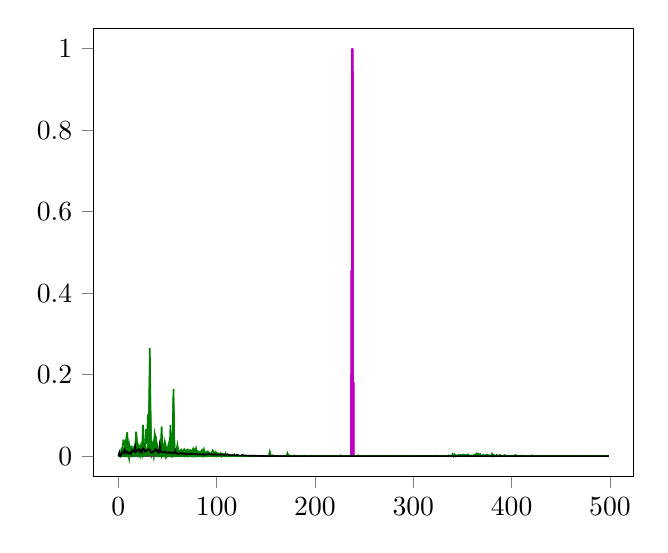
\begin{tikzpicture}

\definecolor{color0}{rgb}{0.75,0,0.75}

\begin{axis}[
xmin=-24.95, xmax=523.95,
ymin=-0.05, ymax=1.05,
tick align=outside,
tick pos=left,
x grid style={lightgray!92.02614379084967!black},
y grid style={lightgray!92.02614379084967!black}
]
\addplot [semithick, color0, forget plot]
table {%
0 0
1 0
2 0
3 0
4 0
5 0
6 0
7 0
8 0
9 0
10 0
11 0
12 0
13 0
14 0
15 0
16 0.002
17 0
18 0
19 0
20 0
21 0
22 0
23 0
24 0
25 0
26 0
27 0
28 0
29 0
30 0
31 0
32 0
33 0
34 0
35 0
36 0
37 0
38 0
39 0
40 0
41 0
42 0
43 0
44 0
45 0
46 0
47 0
48 0
49 0
50 0
51 0
52 0
53 0
54 0
55 0
56 0
57 0
58 0
59 0
60 0
61 0
62 0
63 0
64 0
65 0
66 0
67 0
68 0
69 0
70 0
71 0
72 0
73 0
74 0
75 0
76 0
77 0
78 0
79 0
80 0
81 0
82 0
83 0
84 0
85 0
86 0
87 0
88 0
89 0
90 0
91 0
92 0
93 0
94 0
95 0
96 0
97 0
98 0
99 0
100 0
101 0
102 0
103 0
104 0
105 0
106 0
107 0
108 0
109 0
110 0
111 0
112 0
113 0
114 0
115 0
116 0
117 0
118 0
119 0
120 0
121 0
122 0
123 0
124 0
125 0
126 0
127 0
128 0
129 0
130 0
131 0
132 0
133 0
134 0
135 0
136 0
137 0
138 0
139 0
140 0
141 0
142 0
143 0
144 0
145 0
146 0
147 0
148 0
149 0
150 0
151 0
152 0
153 0
154 0
155 0
156 0
157 0
158 0
159 0
160 0
161 0
162 0
163 0
164 0
165 0
166 0
167 0
168 0
169 0
170 0
171 0
172 0
173 0
174 0
175 0
176 0
177 0
178 0
179 0
180 0
181 0
182 0
183 0
184 0
185 0
186 0
187 0
188 0
189 0
190 0
191 0
192 0
193 0
194 0
195 0
196 0
197 0
198 0
199 0
200 0
201 0
202 0
203 0
204 0
205 0
206 0
207 0
208 0
209 0
210 0
211 0
212 0
213 0
214 0
215 0
216 0
217 0
218 0
219 0
220 0
221 0
222 0
223 0
224 0
225 0
226 0
227 0
228 0
229 0
230 0
231 0
232 0
233 0
234 0
235 0
236 0
237 0
238 0.998
239 0
240 0
241 0
242 0
243 0
244 0
245 0
246 0
247 0
248 0
249 0
250 0
251 0
252 0
253 0
254 0
255 0
256 0
257 0
258 0
259 0
260 0
261 0
262 0
263 0
264 0
265 0
266 0
267 0
268 0
269 0
270 0
271 0
272 0
273 0
274 0
275 0
276 0
277 0
278 0
279 0
280 0
281 0
282 0
283 0
284 0
285 0
286 0
287 0
288 0
289 0
290 0
291 0
292 0
293 0
294 0
295 0
296 0
297 0
298 0
299 0
300 0
301 0
302 0
303 0
304 0
305 0
306 0
307 0
308 0
309 0
310 0
311 0
312 0
313 0
314 0
315 0
316 0
317 0
318 0
319 0
320 0
321 0
322 0
323 0
324 0
325 0
326 0
327 0
328 0
329 0
330 0
331 0
332 0
333 0
334 0
335 0
336 0
337 0
338 0
339 0
340 0
341 0
342 0
343 0
344 0
345 0
346 0
347 0
348 0
349 0
350 0
351 0
352 0
353 0
354 0
355 0
356 0
357 0
358 0
359 0
360 0
361 0
362 0
363 0
364 0
365 0
366 0
367 0
368 0
369 0
370 0
371 0
372 0
373 0
374 0
375 0
376 0
377 0
378 0
379 0
380 0
381 0
382 0
383 0
384 0
385 0
386 0
387 0
388 0
389 0
390 0
391 0
392 0
393 0
394 0
395 0
396 0
397 0
398 0
399 0
400 0
401 0
402 0
403 0
404 0
405 0
406 0
407 0
408 0
409 0
410 0
411 0
412 0
413 0
414 0
415 0
416 0
417 0
418 0
419 0
420 0
421 0
422 0
423 0
424 0
425 0
426 0
427 0
428 0
429 0
430 0
431 0
432 0
433 0
434 0
435 0
436 0
437 0
438 0
439 0
440 0
441 0
442 0
443 0
444 0
445 0
446 0
447 0
448 0
449 0
450 0
451 0
452 0
453 0
454 0
455 0
456 0
457 0
458 0
459 0
460 0
461 0
462 0
463 0
464 0
465 0
466 0
467 0
468 0
469 0
470 0
471 0
472 0
473 0
474 0
475 0
476 0
477 0
478 0
479 0
480 0
481 0
482 0
483 0
484 0
485 0
486 0
487 0
488 0
489 0
490 0
491 0
492 0
493 0
494 0
495 0
496 0
497 0
498 0
499 0
};
\addplot [semithick, color0, forget plot]
table {%
0 0
1 0
2 0
3 0
4 0
5 0
6 0
7 0
8 0
9 0
10 0
11 0
12 0
13 0
14 0
15 0
16 0
17 0
18 0
19 0
20 0
21 0
22 0
23 0
24 0
25 0
26 0
27 0
28 0
29 0
30 0
31 0
32 0
33 0
34 0
35 0
36 0
37 0
38 0
39 0
40 0
41 0
42 0
43 0
44 0
45 0
46 0
47 0
48 0
49 0
50 0
51 0
52 0
53 0
54 0
55 0
56 0
57 0
58 0
59 0
60 0
61 0
62 0
63 0
64 0
65 0
66 0
67 0
68 0
69 0
70 0
71 0
72 0
73 0
74 0
75 0
76 0
77 0
78 0
79 0
80 0
81 0
82 0
83 0
84 0
85 0
86 0
87 0
88 0
89 0
90 0
91 0
92 0
93 0
94 0
95 0
96 0
97 0
98 0
99 0
100 0
101 0
102 0
103 0
104 0
105 0
106 0
107 0
108 0
109 0
110 0
111 0
112 0
113 0
114 0
115 0
116 0
117 0
118 0
119 0
120 0
121 0
122 0
123 0
124 0
125 0
126 0
127 0
128 0
129 0
130 0
131 0
132 0
133 0
134 0
135 0
136 0
137 0
138 0
139 0
140 0
141 0
142 0
143 0
144 0
145 0
146 0
147 0
148 0
149 0
150 0
151 0
152 0
153 0
154 0
155 0
156 0
157 0
158 0
159 0
160 0
161 0
162 0
163 0
164 0
165 0
166 0
167 0
168 0
169 0
170 0
171 0
172 0
173 0
174 0
175 0
176 0
177 0
178 0
179 0
180 0
181 0
182 0
183 0
184 0
185 0
186 0
187 0
188 0
189 0
190 0
191 0
192 0
193 0
194 0
195 0
196 0
197 0
198 0
199 0
200 0
201 0
202 0
203 0
204 0
205 0
206 0
207 0
208 0
209 0
210 0
211 0
212 0
213 0
214 0
215 0
216 0
217 0
218 0
219 0
220 0
221 0
222 0
223 0
224 0
225 0
226 0
227 0
228 0
229 0
230 0
231 0
232 0
233 0
234 0
235 0
236 0
237 0
238 1
239 0
240 0
241 0
242 0
243 0
244 0
245 0
246 0
247 0
248 0
249 0
250 0
251 0
252 0
253 0
254 0
255 0
256 0
257 0
258 0
259 0
260 0
261 0
262 0
263 0
264 0
265 0
266 0
267 0
268 0
269 0
270 0
271 0
272 0
273 0
274 0
275 0
276 0
277 0
278 0
279 0
280 0
281 0
282 0
283 0
284 0
285 0
286 0
287 0
288 0
289 0
290 0
291 0
292 0
293 0
294 0
295 0
296 0
297 0
298 0
299 0
300 0
301 0
302 0
303 0
304 0
305 0
306 0
307 0
308 0
309 0
310 0
311 0
312 0
313 0
314 0
315 0
316 0
317 0
318 0
319 0
320 0
321 0
322 0
323 0
324 0
325 0
326 0
327 0
328 0
329 0
330 0
331 0
332 0
333 0
334 0
335 0
336 0
337 0
338 0
339 0
340 0
341 0
342 0
343 0
344 0
345 0
346 0
347 0
348 0
349 0
350 0
351 0
352 0
353 0
354 0
355 0
356 0
357 0
358 0
359 0
360 0
361 0
362 0
363 0
364 0
365 0
366 0
367 0
368 0
369 0
370 0
371 0
372 0
373 0
374 0
375 0
376 0
377 0
378 0
379 0
380 0
381 0
382 0
383 0
384 0
385 0
386 0
387 0
388 0
389 0
390 0
391 0
392 0
393 0
394 0
395 0
396 0
397 0
398 0
399 0
400 0
401 0
402 0
403 0
404 0
405 0
406 0
407 0
408 0
409 0
410 0
411 0
412 0
413 0
414 0
415 0
416 0
417 0
418 0
419 0
420 0
421 0
422 0
423 0
424 0
425 0
426 0
427 0
428 0
429 0
430 0
431 0
432 0
433 0
434 0
435 0
436 0
437 0
438 0
439 0
440 0
441 0
442 0
443 0
444 0
445 0
446 0
447 0
448 0
449 0
450 0
451 0
452 0
453 0
454 0
455 0
456 0
457 0
458 0
459 0
460 0
461 0
462 0
463 0
464 0
465 0
466 0
467 0
468 0
469 0
470 0
471 0
472 0
473 0
474 0
475 0
476 0
477 0
478 0
479 0
480 0
481 0
482 0
483 0
484 0
485 0
486 0
487 0
488 0
489 0
490 0
491 0
492 0
493 0
494 0
495 0
496 0
497 0
498 0
499 0
};
\addplot [semithick, color0, forget plot]
table {%
0 0
1 0
2 0
3 0
4 0
5 0
6 0
7 0
8 0
9 0
10 0
11 0
12 0
13 0
14 0
15 0
16 0
17 0
18 0
19 0
20 0
21 0
22 0
23 0
24 0
25 0
26 0
27 0
28 0
29 0
30 0
31 0
32 0
33 0
34 0
35 0
36 0
37 0
38 0
39 0
40 0
41 0
42 0
43 0
44 0
45 0
46 0
47 0
48 0
49 0
50 0
51 0
52 0
53 0
54 0
55 0
56 0
57 0
58 0
59 0
60 0
61 0
62 0
63 0
64 0
65 0
66 0
67 0
68 0
69 0
70 0
71 0
72 0
73 0
74 0
75 0
76 0
77 0
78 0
79 0
80 0
81 0
82 0
83 0
84 0
85 0
86 0
87 0
88 0
89 0
90 0
91 0
92 0
93 0
94 0
95 0
96 0
97 0
98 0
99 0
100 0
101 0
102 0
103 0
104 0
105 0
106 0
107 0
108 0
109 0
110 0
111 0
112 0
113 0
114 0
115 0
116 0
117 0
118 0
119 0
120 0
121 0
122 0
123 0
124 0
125 0
126 0
127 0
128 0
129 0
130 0
131 0
132 0
133 0
134 0
135 0
136 0
137 0
138 0
139 0
140 0
141 0
142 0
143 0
144 0
145 0
146 0
147 0
148 0
149 0
150 0
151 0
152 0
153 0
154 0
155 0
156 0
157 0
158 0
159 0
160 0
161 0
162 0
163 0
164 0
165 0
166 0
167 0
168 0
169 0
170 0
171 0
172 0
173 0
174 0
175 0
176 0
177 0
178 0
179 0
180 0
181 0
182 0
183 0
184 0
185 0
186 0
187 0
188 0
189 0
190 0
191 0
192 0
193 0
194 0
195 0
196 0
197 0
198 0
199 0
200 0
201 0
202 0
203 0
204 0
205 0
206 0
207 0
208 0
209 0
210 0
211 0
212 0
213 0
214 0
215 0
216 0
217 0
218 0
219 0
220 0
221 0
222 0
223 0
224 0
225 0
226 0
227 0
228 0
229 0
230 0
231 0
232 0
233 0
234 0
235 0
236 0
237 0
238 1
239 0
240 0
241 0
242 0
243 0
244 0
245 0
246 0
247 0
248 0
249 0
250 0
251 0
252 0
253 0
254 0
255 0
256 0
257 0
258 0
259 0
260 0
261 0
262 0
263 0
264 0
265 0
266 0
267 0
268 0
269 0
270 0
271 0
272 0
273 0
274 0
275 0
276 0
277 0
278 0
279 0
280 0
281 0
282 0
283 0
284 0
285 0
286 0
287 0
288 0
289 0
290 0
291 0
292 0
293 0
294 0
295 0
296 0
297 0
298 0
299 0
300 0
301 0
302 0
303 0
304 0
305 0
306 0
307 0
308 0
309 0
310 0
311 0
312 0
313 0
314 0
315 0
316 0
317 0
318 0
319 0
320 0
321 0
322 0
323 0
324 0
325 0
326 0
327 0
328 0
329 0
330 0
331 0
332 0
333 0
334 0
335 0
336 0
337 0
338 0
339 0
340 0
341 0
342 0
343 0
344 0
345 0
346 0
347 0
348 0
349 0
350 0
351 0
352 0
353 0
354 0
355 0
356 0
357 0
358 0
359 0
360 0
361 0
362 0
363 0
364 0
365 0
366 0
367 0
368 0
369 0
370 0
371 0
372 0
373 0
374 0
375 0
376 0
377 0
378 0
379 0
380 0
381 0
382 0
383 0
384 0
385 0
386 0
387 0
388 0
389 0
390 0
391 0
392 0
393 0
394 0
395 0
396 0
397 0
398 0
399 0
400 0
401 0
402 0
403 0
404 0
405 0
406 0
407 0
408 0
409 0
410 0
411 0
412 0
413 0
414 0
415 0
416 0
417 0
418 0
419 0
420 0
421 0
422 0
423 0
424 0
425 0
426 0
427 0
428 0
429 0
430 0
431 0
432 0
433 0
434 0
435 0
436 0
437 0
438 0
439 0
440 0
441 0
442 0
443 0
444 0
445 0
446 0
447 0
448 0
449 0
450 0
451 0
452 0
453 0
454 0
455 0
456 0
457 0
458 0
459 0
460 0
461 0
462 0
463 0
464 0
465 0
466 0
467 0
468 0
469 0
470 0
471 0
472 0
473 0
474 0
475 0
476 0
477 0
478 0
479 0
480 0
481 0
482 0
483 0
484 0
485 0
486 0
487 0
488 0
489 0
490 0
491 0
492 0
493 0
494 0
495 0
496 0
497 0
498 0
499 0
};
\addplot [semithick, color0, forget plot]
table {%
0 0
1 0
2 0
3 0
4 0
5 0
6 0
7 0
8 0
9 0
10 0
11 0
12 0
13 0
14 0
15 0
16 0
17 0
18 0
19 0
20 0
21 0
22 0
23 0
24 0
25 0
26 0
27 0
28 0
29 0
30 0
31 0
32 0
33 0
34 0
35 0
36 0
37 0
38 0
39 0
40 0
41 0
42 0
43 0
44 0
45 0
46 0
47 0
48 0
49 0
50 0
51 0
52 0
53 0
54 0
55 0
56 0
57 0
58 0
59 0
60 0
61 0
62 0
63 0
64 0
65 0
66 0
67 0
68 0
69 0
70 0
71 0
72 0
73 0
74 0
75 0
76 0
77 0
78 0
79 0
80 0
81 0
82 0
83 0
84 0
85 0
86 0
87 0
88 0
89 0
90 0
91 0
92 0
93 0
94 0
95 0
96 0
97 0
98 0
99 0
100 0
101 0
102 0
103 0
104 0
105 0
106 0
107 0
108 0
109 0
110 0
111 0
112 0
113 0
114 0
115 0
116 0
117 0
118 0
119 0
120 0
121 0
122 0
123 0
124 0
125 0
126 0
127 0
128 0
129 0
130 0
131 0
132 0
133 0
134 0
135 0
136 0
137 0
138 0
139 0
140 0
141 0
142 0
143 0
144 0
145 0
146 0
147 0
148 0
149 0
150 0
151 0
152 0
153 0
154 0
155 0
156 0
157 0
158 0
159 0
160 0
161 0
162 0
163 0
164 0
165 0
166 0
167 0
168 0
169 0
170 0
171 0
172 0
173 0
174 0
175 0
176 0
177 0
178 0
179 0
180 0
181 0
182 0
183 0
184 0
185 0
186 0
187 0
188 0
189 0
190 0
191 0
192 0
193 0
194 0
195 0
196 0
197 0
198 0
199 0
200 0
201 0
202 0
203 0
204 0
205 0
206 0
207 0
208 0
209 0
210 0
211 0
212 0
213 0
214 0
215 0
216 0
217 0
218 0
219 0
220 0
221 0
222 0
223 0
224 0
225 0
226 0
227 0
228 0
229 0
230 0
231 0
232 0
233 0
234 0
235 0
236 0
237 0
238 1
239 0
240 0
241 0
242 0
243 0
244 0
245 0
246 0
247 0
248 0
249 0
250 0
251 0
252 0
253 0
254 0
255 0
256 0
257 0
258 0
259 0
260 0
261 0
262 0
263 0
264 0
265 0
266 0
267 0
268 0
269 0
270 0
271 0
272 0
273 0
274 0
275 0
276 0
277 0
278 0
279 0
280 0
281 0
282 0
283 0
284 0
285 0
286 0
287 0
288 0
289 0
290 0
291 0
292 0
293 0
294 0
295 0
296 0
297 0
298 0
299 0
300 0
301 0
302 0
303 0
304 0
305 0
306 0
307 0
308 0
309 0
310 0
311 0
312 0
313 0
314 0
315 0
316 0
317 0
318 0
319 0
320 0
321 0
322 0
323 0
324 0
325 0
326 0
327 0
328 0
329 0
330 0
331 0
332 0
333 0
334 0
335 0
336 0
337 0
338 0
339 0
340 0
341 0
342 0
343 0
344 0
345 0
346 0
347 0
348 0
349 0
350 0
351 0
352 0
353 0
354 0
355 0
356 0
357 0
358 0
359 0
360 0
361 0
362 0
363 0
364 0
365 0
366 0
367 0
368 0
369 0
370 0
371 0
372 0
373 0
374 0
375 0
376 0
377 0
378 0
379 0
380 0
381 0
382 0
383 0
384 0
385 0
386 0
387 0
388 0
389 0
390 0
391 0
392 0
393 0
394 0
395 0
396 0
397 0
398 0
399 0
400 0
401 0
402 0
403 0
404 0
405 0
406 0
407 0
408 0
409 0
410 0
411 0
412 0
413 0
414 0
415 0
416 0
417 0
418 0
419 0
420 0
421 0
422 0
423 0
424 0
425 0
426 0
427 0
428 0
429 0
430 0
431 0
432 0
433 0
434 0
435 0
436 0
437 0
438 0
439 0
440 0
441 0
442 0
443 0
444 0
445 0
446 0
447 0
448 0
449 0
450 0
451 0
452 0
453 0
454 0
455 0
456 0
457 0
458 0
459 0
460 0
461 0
462 0
463 0
464 0
465 0
466 0
467 0
468 0
469 0
470 0
471 0
472 0
473 0
474 0
475 0
476 0
477 0
478 0
479 0
480 0
481 0
482 0
483 0
484 0
485 0
486 0
487 0
488 0
489 0
490 0
491 0
492 0
493 0
494 0
495 0
496 0
497 0
498 0
499 0
};
\addplot [semithick, color0, forget plot]
table {%
0 0
1 0
2 0
3 0
4 0
5 0
6 0
7 0
8 0
9 0
10 0
11 0
12 0
13 0
14 0
15 0
16 0
17 0
18 0
19 0
20 0
21 0
22 0
23 0
24 0
25 0
26 0
27 0
28 0
29 0
30 0
31 0
32 0
33 0
34 0
35 0
36 0
37 0
38 0
39 0
40 0
41 0
42 0
43 0
44 0
45 0
46 0
47 0
48 0
49 0
50 0
51 0
52 0
53 0
54 0
55 0
56 0
57 0
58 0
59 0
60 0
61 0
62 0
63 0
64 0
65 0
66 0
67 0
68 0
69 0
70 0
71 0
72 0
73 0
74 0
75 0
76 0
77 0
78 0
79 0
80 0
81 0
82 0
83 0
84 0
85 0
86 0
87 0
88 0
89 0
90 0
91 0
92 0
93 0
94 0
95 0
96 0
97 0
98 0
99 0
100 0
101 0
102 0
103 0
104 0
105 0
106 0
107 0
108 0
109 0
110 0
111 0
112 0
113 0
114 0
115 0
116 0
117 0
118 0
119 0
120 0
121 0
122 0
123 0
124 0
125 0
126 0
127 0
128 0
129 0
130 0
131 0
132 0
133 0
134 0
135 0
136 0
137 0
138 0
139 0
140 0
141 0
142 0
143 0
144 0
145 0
146 0
147 0
148 0
149 0
150 0
151 0
152 0
153 0
154 0
155 0
156 0
157 0
158 0
159 0
160 0
161 0
162 0
163 0
164 0
165 0
166 0
167 0
168 0
169 0
170 0
171 0
172 0
173 0
174 0
175 0
176 0
177 0
178 0
179 0
180 0
181 0
182 0
183 0
184 0
185 0
186 0
187 0
188 0
189 0
190 0
191 0
192 0
193 0
194 0
195 0
196 0
197 0
198 0
199 0
200 0
201 0
202 0
203 0
204 0
205 0
206 0
207 0
208 0
209 0
210 0
211 0
212 0
213 0
214 0
215 0
216 0
217 0
218 0
219 0
220 0
221 0
222 0
223 0
224 0
225 0
226 0
227 0
228 0
229 0
230 0
231 0
232 0
233 0
234 0
235 0
236 0
237 0
238 1
239 0
240 0
241 0
242 0
243 0
244 0
245 0
246 0
247 0
248 0
249 0
250 0
251 0
252 0
253 0
254 0
255 0
256 0
257 0
258 0
259 0
260 0
261 0
262 0
263 0
264 0
265 0
266 0
267 0
268 0
269 0
270 0
271 0
272 0
273 0
274 0
275 0
276 0
277 0
278 0
279 0
280 0
281 0
282 0
283 0
284 0
285 0
286 0
287 0
288 0
289 0
290 0
291 0
292 0
293 0
294 0
295 0
296 0
297 0
298 0
299 0
300 0
301 0
302 0
303 0
304 0
305 0
306 0
307 0
308 0
309 0
310 0
311 0
312 0
313 0
314 0
315 0
316 0
317 0
318 0
319 0
320 0
321 0
322 0
323 0
324 0
325 0
326 0
327 0
328 0
329 0
330 0
331 0
332 0
333 0
334 0
335 0
336 0
337 0
338 0
339 0
340 0
341 0
342 0
343 0
344 0
345 0
346 0
347 0
348 0
349 0
350 0
351 0
352 0
353 0
354 0
355 0
356 0
357 0
358 0
359 0
360 0
361 0
362 0
363 0
364 0
365 0
366 0
367 0
368 0
369 0
370 0
371 0
372 0
373 0
374 0
375 0
376 0
377 0
378 0
379 0
380 0
381 0
382 0
383 0
384 0
385 0
386 0
387 0
388 0
389 0
390 0
391 0
392 0
393 0
394 0
395 0
396 0
397 0
398 0
399 0
400 0
401 0
402 0
403 0
404 0
405 0
406 0
407 0
408 0
409 0
410 0
411 0
412 0
413 0
414 0
415 0
416 0
417 0
418 0
419 0
420 0
421 0
422 0
423 0
424 0
425 0
426 0
427 0
428 0
429 0
430 0
431 0
432 0
433 0
434 0
435 0
436 0
437 0
438 0
439 0
440 0
441 0
442 0
443 0
444 0
445 0
446 0
447 0
448 0
449 0
450 0
451 0
452 0
453 0
454 0
455 0
456 0
457 0
458 0
459 0
460 0
461 0
462 0
463 0
464 0
465 0
466 0
467 0
468 0
469 0
470 0
471 0
472 0
473 0
474 0
475 0
476 0
477 0
478 0
479 0
480 0
481 0
482 0
483 0
484 0
485 0
486 0
487 0
488 0
489 0
490 0
491 0
492 0
493 0
494 0
495 0
496 0
497 0
498 0
499 0
};
\addplot [semithick, color0, forget plot]
table {%
0 0
1 0
2 0
3 0
4 0
5 0
6 0
7 0
8 0
9 0
10 0
11 0
12 0
13 0
14 0
15 0
16 0
17 0
18 0
19 0
20 0
21 0
22 0
23 0
24 0
25 0
26 0
27 0
28 0
29 0
30 0
31 0
32 0
33 0
34 0
35 0
36 0
37 0
38 0
39 0
40 0
41 0
42 0
43 0
44 0
45 0
46 0
47 0
48 0
49 0
50 0
51 0
52 0
53 0
54 0
55 0
56 0
57 0
58 0
59 0
60 0
61 0
62 0
63 0
64 0
65 0
66 0
67 0
68 0
69 0
70 0
71 0
72 0
73 0
74 0
75 0
76 0
77 0
78 0
79 0
80 0
81 0
82 0
83 0
84 0
85 0
86 0
87 0
88 0
89 0
90 0
91 0
92 0
93 0
94 0
95 0
96 0
97 0
98 0
99 0
100 0
101 0
102 0
103 0
104 0
105 0
106 0
107 0
108 0
109 0
110 0
111 0
112 0
113 0
114 0
115 0
116 0
117 0
118 0
119 0
120 0
121 0
122 0
123 0
124 0
125 0
126 0
127 0
128 0
129 0
130 0
131 0
132 0
133 0
134 0
135 0
136 0
137 0
138 0
139 0
140 0
141 0
142 0
143 0
144 0
145 0
146 0
147 0
148 0
149 0
150 0
151 0
152 0
153 0
154 0
155 0
156 0
157 0
158 0
159 0
160 0
161 0
162 0
163 0
164 0
165 0
166 0
167 0
168 0
169 0
170 0
171 0
172 0
173 0
174 0
175 0
176 0
177 0
178 0
179 0
180 0
181 0
182 0
183 0
184 0
185 0
186 0
187 0
188 0
189 0
190 0
191 0
192 0
193 0
194 0
195 0
196 0
197 0
198 0
199 0
200 0
201 0
202 0
203 0
204 0
205 0
206 0
207 0
208 0
209 0
210 0
211 0
212 0
213 0
214 0
215 0
216 0
217 0
218 0
219 0
220 0
221 0
222 0
223 0
224 0
225 0
226 0
227 0
228 0
229 0
230 0
231 0
232 0
233 0
234 0
235 0
236 0
237 0
238 1
239 0
240 0
241 0
242 0
243 0
244 0
245 0
246 0
247 0
248 0
249 0
250 0
251 0
252 0
253 0
254 0
255 0
256 0
257 0
258 0
259 0
260 0
261 0
262 0
263 0
264 0
265 0
266 0
267 0
268 0
269 0
270 0
271 0
272 0
273 0
274 0
275 0
276 0
277 0
278 0
279 0
280 0
281 0
282 0
283 0
284 0
285 0
286 0
287 0
288 0
289 0
290 0
291 0
292 0
293 0
294 0
295 0
296 0
297 0
298 0
299 0
300 0
301 0
302 0
303 0
304 0
305 0
306 0
307 0
308 0
309 0
310 0
311 0
312 0
313 0
314 0
315 0
316 0
317 0
318 0
319 0
320 0
321 0
322 0
323 0
324 0
325 0
326 0
327 0
328 0
329 0
330 0
331 0
332 0
333 0
334 0
335 0
336 0
337 0
338 0
339 0
340 0
341 0
342 0
343 0
344 0
345 0
346 0
347 0
348 0
349 0
350 0
351 0
352 0
353 0
354 0
355 0
356 0
357 0
358 0
359 0
360 0
361 0
362 0
363 0
364 0
365 0
366 0
367 0
368 0
369 0
370 0
371 0
372 0
373 0
374 0
375 0
376 0
377 0
378 0
379 0
380 0
381 0
382 0
383 0
384 0
385 0
386 0
387 0
388 0
389 0
390 0
391 0
392 0
393 0
394 0
395 0
396 0
397 0
398 0
399 0
400 0
401 0
402 0
403 0
404 0
405 0
406 0
407 0
408 0
409 0
410 0
411 0
412 0
413 0
414 0
415 0
416 0
417 0
418 0
419 0
420 0
421 0
422 0
423 0
424 0
425 0
426 0
427 0
428 0
429 0
430 0
431 0
432 0
433 0
434 0
435 0
436 0
437 0
438 0
439 0
440 0
441 0
442 0
443 0
444 0
445 0
446 0
447 0
448 0
449 0
450 0
451 0
452 0
453 0
454 0
455 0
456 0
457 0
458 0
459 0
460 0
461 0
462 0
463 0
464 0
465 0
466 0
467 0
468 0
469 0
470 0
471 0
472 0
473 0
474 0
475 0
476 0
477 0
478 0
479 0
480 0
481 0
482 0
483 0
484 0
485 0
486 0
487 0
488 0
489 0
490 0
491 0
492 0
493 0
494 0
495 0
496 0
497 0
498 0
499 0
};
\addplot [semithick, color0, forget plot]
table {%
0 0
1 0
2 0
3 0
4 0
5 0
6 0
7 0
8 0
9 0
10 0
11 0
12 0
13 0
14 0
15 0
16 0
17 0
18 0
19 0
20 0
21 0
22 0
23 0
24 0
25 0
26 0
27 0
28 0
29 0
30 0
31 0
32 0
33 0
34 0
35 0
36 0
37 0
38 0
39 0
40 0
41 0
42 0
43 0
44 0
45 0
46 0
47 0
48 0
49 0
50 0
51 0
52 0
53 0
54 0
55 0
56 0
57 0
58 0
59 0
60 0
61 0
62 0
63 0
64 0
65 0
66 0
67 0
68 0
69 0
70 0
71 0
72 0
73 0
74 0
75 0
76 0
77 0
78 0
79 0
80 0
81 0
82 0
83 0
84 0
85 0
86 0
87 0
88 0
89 0
90 0
91 0
92 0
93 0
94 0
95 0
96 0
97 0
98 0
99 0
100 0
101 0
102 0
103 0
104 0
105 0
106 0
107 0
108 0
109 0
110 0
111 0
112 0
113 0
114 0
115 0
116 0
117 0
118 0
119 0
120 0
121 0
122 0
123 0
124 0
125 0
126 0
127 0
128 0
129 0
130 0
131 0
132 0
133 0
134 0
135 0
136 0
137 0
138 0
139 0
140 0
141 0
142 0
143 0
144 0
145 0
146 0
147 0
148 0
149 0
150 0
151 0
152 0
153 0
154 0
155 0
156 0
157 0
158 0
159 0
160 0
161 0
162 0
163 0
164 0
165 0
166 0
167 0
168 0
169 0
170 0
171 0
172 0
173 0
174 0
175 0
176 0
177 0
178 0
179 0
180 0
181 0
182 0
183 0
184 0
185 0
186 0
187 0
188 0
189 0
190 0
191 0
192 0
193 0
194 0
195 0
196 0
197 0
198 0
199 0
200 0
201 0
202 0
203 0
204 0
205 0
206 0
207 0
208 0
209 0
210 0
211 0
212 0
213 0
214 0
215 0
216 0
217 0
218 0
219 0
220 0
221 0
222 0
223 0
224 0
225 0
226 0
227 0
228 0
229 0
230 0
231 0
232 0
233 0
234 0
235 0
236 0
237 0
238 1
239 0
240 0
241 0
242 0
243 0
244 0
245 0
246 0
247 0
248 0
249 0
250 0
251 0
252 0
253 0
254 0
255 0
256 0
257 0
258 0
259 0
260 0
261 0
262 0
263 0
264 0
265 0
266 0
267 0
268 0
269 0
270 0
271 0
272 0
273 0
274 0
275 0
276 0
277 0
278 0
279 0
280 0
281 0
282 0
283 0
284 0
285 0
286 0
287 0
288 0
289 0
290 0
291 0
292 0
293 0
294 0
295 0
296 0
297 0
298 0
299 0
300 0
301 0
302 0
303 0
304 0
305 0
306 0
307 0
308 0
309 0
310 0
311 0
312 0
313 0
314 0
315 0
316 0
317 0
318 0
319 0
320 0
321 0
322 0
323 0
324 0
325 0
326 0
327 0
328 0
329 0
330 0
331 0
332 0
333 0
334 0
335 0
336 0
337 0
338 0
339 0
340 0
341 0
342 0
343 0
344 0
345 0
346 0
347 0
348 0
349 0
350 0
351 0
352 0
353 0
354 0
355 0
356 0
357 0
358 0
359 0
360 0
361 0
362 0
363 0
364 0
365 0
366 0
367 0
368 0
369 0
370 0
371 0
372 0
373 0
374 0
375 0
376 0
377 0
378 0
379 0
380 0
381 0
382 0
383 0
384 0
385 0
386 0
387 0
388 0
389 0
390 0
391 0
392 0
393 0
394 0
395 0
396 0
397 0
398 0
399 0
400 0
401 0
402 0
403 0
404 0
405 0
406 0
407 0
408 0
409 0
410 0
411 0
412 0
413 0
414 0
415 0
416 0
417 0
418 0
419 0
420 0
421 0
422 0
423 0
424 0
425 0
426 0
427 0
428 0
429 0
430 0
431 0
432 0
433 0
434 0
435 0
436 0
437 0
438 0
439 0
440 0
441 0
442 0
443 0
444 0
445 0
446 0
447 0
448 0
449 0
450 0
451 0
452 0
453 0
454 0
455 0
456 0
457 0
458 0
459 0
460 0
461 0
462 0
463 0
464 0
465 0
466 0
467 0
468 0
469 0
470 0
471 0
472 0
473 0
474 0
475 0
476 0
477 0
478 0
479 0
480 0
481 0
482 0
483 0
484 0
485 0
486 0
487 0
488 0
489 0
490 0
491 0
492 0
493 0
494 0
495 0
496 0
497 0
498 0
499 0
};
\addplot [semithick, color0, forget plot]
table {%
0 0
1 0
2 0
3 0
4 0
5 0
6 0
7 0
8 0
9 0
10 0
11 0
12 0
13 0
14 0
15 0
16 0
17 0
18 0
19 0
20 0
21 0
22 0
23 0
24 0
25 0
26 0
27 0
28 0
29 0
30 0
31 0
32 0
33 0
34 0
35 0
36 0
37 0
38 0
39 0
40 0
41 0
42 0
43 0
44 0
45 0
46 0
47 0
48 0
49 0
50 0
51 0
52 0
53 0
54 0
55 0
56 0
57 0
58 0
59 0
60 0
61 0
62 0
63 0
64 0
65 0
66 0
67 0
68 0
69 0
70 0
71 0
72 0
73 0
74 0
75 0
76 0
77 0
78 0
79 0
80 0
81 0
82 0
83 0
84 0
85 0
86 0
87 0
88 0
89 0
90 0
91 0
92 0
93 0
94 0
95 0
96 0
97 0
98 0
99 0
100 0
101 0
102 0
103 0
104 0
105 0
106 0
107 0
108 0
109 0
110 0
111 0
112 0
113 0
114 0
115 0
116 0
117 0
118 0
119 0
120 0
121 0
122 0
123 0
124 0
125 0
126 0
127 0
128 0
129 0
130 0
131 0
132 0
133 0
134 0
135 0
136 0
137 0
138 0
139 0
140 0
141 0
142 0
143 0
144 0
145 0
146 0
147 0
148 0
149 0
150 0
151 0
152 0
153 0
154 0
155 0
156 0
157 0
158 0
159 0
160 0
161 0
162 0
163 0
164 0
165 0
166 0
167 0
168 0
169 0
170 0
171 0
172 0
173 0
174 0
175 0
176 0
177 0
178 0
179 0
180 0
181 0
182 0
183 0
184 0
185 0
186 0
187 0
188 0
189 0
190 0
191 0
192 0
193 0
194 0
195 0
196 0
197 0
198 0
199 0
200 0
201 0
202 0
203 0
204 0
205 0
206 0
207 0
208 0
209 0
210 0
211 0
212 0
213 0
214 0
215 0
216 0
217 0
218 0
219 0
220 0
221 0
222 0
223 0
224 0
225 0
226 0
227 0
228 0
229 0
230 0
231 0
232 0
233 0
234 0
235 0
236 0
237 0
238 1
239 0
240 0
241 0
242 0
243 0
244 0
245 0
246 0
247 0
248 0
249 0
250 0
251 0
252 0
253 0
254 0
255 0
256 0
257 0
258 0
259 0
260 0
261 0
262 0
263 0
264 0
265 0
266 0
267 0
268 0
269 0
270 0
271 0
272 0
273 0
274 0
275 0
276 0
277 0
278 0
279 0
280 0
281 0
282 0
283 0
284 0
285 0
286 0
287 0
288 0
289 0
290 0
291 0
292 0
293 0
294 0
295 0
296 0
297 0
298 0
299 0
300 0
301 0
302 0
303 0
304 0
305 0
306 0
307 0
308 0
309 0
310 0
311 0
312 0
313 0
314 0
315 0
316 0
317 0
318 0
319 0
320 0
321 0
322 0
323 0
324 0
325 0
326 0
327 0
328 0
329 0
330 0
331 0
332 0
333 0
334 0
335 0
336 0
337 0
338 0
339 0
340 0
341 0
342 0
343 0
344 0
345 0
346 0
347 0
348 0
349 0
350 0
351 0
352 0
353 0
354 0
355 0
356 0
357 0
358 0
359 0
360 0
361 0
362 0
363 0
364 0
365 0
366 0
367 0
368 0
369 0
370 0
371 0
372 0
373 0
374 0
375 0
376 0
377 0
378 0
379 0
380 0
381 0
382 0
383 0
384 0
385 0
386 0
387 0
388 0
389 0
390 0
391 0
392 0
393 0
394 0
395 0
396 0
397 0
398 0
399 0
400 0
401 0
402 0
403 0
404 0
405 0
406 0
407 0
408 0
409 0
410 0
411 0
412 0
413 0
414 0
415 0
416 0
417 0
418 0
419 0
420 0
421 0
422 0
423 0
424 0
425 0
426 0
427 0
428 0
429 0
430 0
431 0
432 0
433 0
434 0
435 0
436 0
437 0
438 0
439 0
440 0
441 0
442 0
443 0
444 0
445 0
446 0
447 0
448 0
449 0
450 0
451 0
452 0
453 0
454 0
455 0
456 0
457 0
458 0
459 0
460 0
461 0
462 0
463 0
464 0
465 0
466 0
467 0
468 0
469 0
470 0
471 0
472 0
473 0
474 0
475 0
476 0
477 0
478 0
479 0
480 0
481 0
482 0
483 0
484 0
485 0
486 0
487 0
488 0
489 0
490 0
491 0
492 0
493 0
494 0
495 0
496 0
497 0
498 0
499 0
};
\addplot [semithick, color0, forget plot]
table {%
0 0
1 0
2 0
3 0
4 0
5 0
6 0
7 0
8 0
9 0
10 0
11 0
12 0
13 0
14 0
15 0
16 0
17 0
18 0
19 0
20 0
21 0
22 0
23 0
24 0
25 0
26 0
27 0
28 0
29 0
30 0
31 0
32 0
33 0
34 0
35 0
36 0
37 0
38 0
39 0
40 0
41 0
42 0
43 0
44 0
45 0
46 0
47 0
48 0
49 0
50 0
51 0
52 0
53 0
54 0
55 0
56 0
57 0
58 0
59 0
60 0
61 0
62 0
63 0
64 0
65 0
66 0
67 0
68 0
69 0
70 0
71 0
72 0
73 0
74 0
75 0
76 0
77 0
78 0
79 0
80 0
81 0
82 0
83 0
84 0
85 0
86 0
87 0
88 0
89 0
90 0
91 0
92 0
93 0
94 0
95 0
96 0
97 0
98 0
99 0
100 0
101 0
102 0
103 0
104 0
105 0
106 0
107 0
108 0
109 0
110 0
111 0
112 0
113 0
114 0
115 0
116 0
117 0
118 0
119 0
120 0
121 0
122 0
123 0
124 0
125 0
126 0
127 0
128 0
129 0
130 0
131 0
132 0
133 0
134 0
135 0
136 0
137 0
138 0
139 0
140 0
141 0
142 0
143 0
144 0
145 0
146 0
147 0
148 0
149 0
150 0
151 0
152 0
153 0
154 0
155 0
156 0
157 0
158 0
159 0
160 0
161 0
162 0
163 0
164 0
165 0
166 0
167 0
168 0
169 0
170 0
171 0
172 0
173 0
174 0
175 0
176 0
177 0
178 0
179 0
180 0
181 0
182 0
183 0
184 0
185 0
186 0
187 0
188 0
189 0
190 0
191 0
192 0
193 0
194 0
195 0
196 0
197 0
198 0
199 0
200 0
201 0
202 0
203 0
204 0
205 0
206 0
207 0
208 0
209 0
210 0
211 0
212 0
213 0
214 0
215 0
216 0
217 0
218 0
219 0
220 0
221 0
222 0
223 0
224 0
225 0
226 0
227 0
228 0
229 0
230 0
231 0
232 0
233 0
234 0
235 0
236 0
237 0
238 1
239 0
240 0
241 0
242 0
243 0
244 0
245 0
246 0
247 0
248 0
249 0
250 0
251 0
252 0
253 0
254 0
255 0
256 0
257 0
258 0
259 0
260 0
261 0
262 0
263 0
264 0
265 0
266 0
267 0
268 0
269 0
270 0
271 0
272 0
273 0
274 0
275 0
276 0
277 0
278 0
279 0
280 0
281 0
282 0
283 0
284 0
285 0
286 0
287 0
288 0
289 0
290 0
291 0
292 0
293 0
294 0
295 0
296 0
297 0
298 0
299 0
300 0
301 0
302 0
303 0
304 0
305 0
306 0
307 0
308 0
309 0
310 0
311 0
312 0
313 0
314 0
315 0
316 0
317 0
318 0
319 0
320 0
321 0
322 0
323 0
324 0
325 0
326 0
327 0
328 0
329 0
330 0
331 0
332 0
333 0
334 0
335 0
336 0
337 0
338 0
339 0
340 0
341 0
342 0
343 0
344 0
345 0
346 0
347 0
348 0
349 0
350 0
351 0
352 0
353 0
354 0
355 0
356 0
357 0
358 0
359 0
360 0
361 0
362 0
363 0
364 0
365 0
366 0
367 0
368 0
369 0
370 0
371 0
372 0
373 0
374 0
375 0
376 0
377 0
378 0
379 0
380 0
381 0
382 0
383 0
384 0
385 0
386 0
387 0
388 0
389 0
390 0
391 0
392 0
393 0
394 0
395 0
396 0
397 0
398 0
399 0
400 0
401 0
402 0
403 0
404 0
405 0
406 0
407 0
408 0
409 0
410 0
411 0
412 0
413 0
414 0
415 0
416 0
417 0
418 0
419 0
420 0
421 0
422 0
423 0
424 0
425 0
426 0
427 0
428 0
429 0
430 0
431 0
432 0
433 0
434 0
435 0
436 0
437 0
438 0
439 0
440 0
441 0
442 0
443 0
444 0
445 0
446 0
447 0
448 0
449 0
450 0
451 0
452 0
453 0
454 0
455 0
456 0
457 0
458 0
459 0
460 0
461 0
462 0
463 0
464 0
465 0
466 0
467 0
468 0
469 0
470 0
471 0
472 0
473 0
474 0
475 0
476 0
477 0
478 0
479 0
480 0
481 0
482 0
483 0
484 0
485 0
486 0
487 0
488 0
489 0
490 0
491 0
492 0
493 0
494 0
495 0
496 0
497 0
498 0
499 0
};
\addplot [semithick, color0, forget plot]
table {%
0 0
1 0
2 0
3 0
4 0
5 0
6 0
7 0
8 0
9 0
10 0
11 0
12 0
13 0
14 0
15 0
16 0
17 0
18 0
19 0
20 0
21 0
22 0
23 0
24 0
25 0
26 0
27 0
28 0
29 0
30 0
31 0
32 0
33 0
34 0
35 0
36 0
37 0
38 0
39 0
40 0
41 0
42 0
43 0
44 0
45 0
46 0
47 0
48 0
49 0
50 0
51 0
52 0
53 0
54 0
55 0
56 0
57 0
58 0
59 0
60 0
61 0
62 0
63 0
64 0
65 0
66 0
67 0
68 0
69 0
70 0
71 0
72 0
73 0
74 0
75 0
76 0
77 0
78 0
79 0
80 0
81 0
82 0
83 0
84 0
85 0
86 0
87 0
88 0
89 0
90 0
91 0
92 0
93 0
94 0
95 0
96 0
97 0
98 0
99 0
100 0
101 0
102 0
103 0
104 0
105 0
106 0
107 0
108 0
109 0
110 0
111 0
112 0
113 0
114 0
115 0
116 0
117 0
118 0
119 0
120 0
121 0
122 0
123 0
124 0
125 0
126 0
127 0
128 0
129 0
130 0
131 0
132 0
133 0
134 0
135 0
136 0
137 0
138 0
139 0
140 0
141 0
142 0
143 0
144 0
145 0
146 0
147 0
148 0
149 0
150 0
151 0
152 0
153 0
154 0
155 0
156 0
157 0
158 0
159 0
160 0
161 0
162 0
163 0
164 0
165 0
166 0
167 0
168 0
169 0
170 0
171 0
172 0
173 0
174 0
175 0
176 0
177 0
178 0
179 0
180 0
181 0
182 0
183 0
184 0
185 0
186 0
187 0
188 0
189 0
190 0
191 0
192 0
193 0
194 0
195 0
196 0
197 0
198 0
199 0
200 0
201 0
202 0
203 0
204 0
205 0
206 0
207 0
208 0
209 0
210 0
211 0
212 0
213 0
214 0
215 0
216 0
217 0
218 0
219 0
220 0
221 0
222 0
223 0
224 0
225 0
226 0
227 0
228 0
229 0
230 0
231 0
232 0
233 0
234 0
235 0
236 0
237 0
238 1
239 0
240 0
241 0
242 0
243 0
244 0
245 0
246 0
247 0
248 0
249 0
250 0
251 0
252 0
253 0
254 0
255 0
256 0
257 0
258 0
259 0
260 0
261 0
262 0
263 0
264 0
265 0
266 0
267 0
268 0
269 0
270 0
271 0
272 0
273 0
274 0
275 0
276 0
277 0
278 0
279 0
280 0
281 0
282 0
283 0
284 0
285 0
286 0
287 0
288 0
289 0
290 0
291 0
292 0
293 0
294 0
295 0
296 0
297 0
298 0
299 0
300 0
301 0
302 0
303 0
304 0
305 0
306 0
307 0
308 0
309 0
310 0
311 0
312 0
313 0
314 0
315 0
316 0
317 0
318 0
319 0
320 0
321 0
322 0
323 0
324 0
325 0
326 0
327 0
328 0
329 0
330 0
331 0
332 0
333 0
334 0
335 0
336 0
337 0
338 0
339 0
340 0
341 0
342 0
343 0
344 0
345 0
346 0
347 0
348 0
349 0
350 0
351 0
352 0
353 0
354 0
355 0
356 0
357 0
358 0
359 0
360 0
361 0
362 0
363 0
364 0
365 0
366 0
367 0
368 0
369 0
370 0
371 0
372 0
373 0
374 0
375 0
376 0
377 0
378 0
379 0
380 0
381 0
382 0
383 0
384 0
385 0
386 0
387 0
388 0
389 0
390 0
391 0
392 0
393 0
394 0
395 0
396 0
397 0
398 0
399 0
400 0
401 0
402 0
403 0
404 0
405 0
406 0
407 0
408 0
409 0
410 0
411 0
412 0
413 0
414 0
415 0
416 0
417 0
418 0
419 0
420 0
421 0
422 0
423 0
424 0
425 0
426 0
427 0
428 0
429 0
430 0
431 0
432 0
433 0
434 0
435 0
436 0
437 0
438 0
439 0
440 0
441 0
442 0
443 0
444 0
445 0
446 0
447 0
448 0
449 0
450 0
451 0
452 0
453 0
454 0
455 0
456 0
457 0
458 0
459 0
460 0
461 0
462 0
463 0
464 0
465 0
466 0
467 0
468 0
469 0
470 0
471 0
472 0
473 0
474 0
475 0
476 0
477 0
478 0
479 0
480 0
481 0
482 0
483 0
484 0
485 0
486 0
487 0
488 0
489 0
490 0
491 0
492 0
493 0
494 0
495 0
496 0
497 0
498 0
499 0
};
\addplot [semithick, green!50.0!black, forget plot]
table {%
0 0
1 0
2 0
3 0
4 0.0101010101010101
5 0.0383838383838384
6 0.0363636363636364
7 0.0222222222222222
8 0.0323232323232323
9 0.0585858585858586
10 0.00606060606060606
11 0.00707070707070707
12 0.0161616161616162
13 0.00505050505050505
14 0.00606060606060606
15 0.0202020202020202
16 0.0151515151515152
17 0.00606060606060606
18 0.00606060606060606
19 0.00909090909090909
20 0.0242424242424242
21 0.0131313131313131
22 0.00202020202020202
23 0.0191919191919192
24 0.0161616161616162
25 0.0141414141414141
26 0.0111111111111111
27 0.00606060606060606
28 0.0181818181818182
29 0.0121212121212121
30 0.00505050505050505
31 0.0141414141414141
32 0.0323232323232323
33 0.0343434343434343
34 0.00303030303030303
35 0.00909090909090909
36 0.00808080808080808
37 0.0171717171717172
38 0.0151515151515152
39 0.0242424242424242
40 0.0111111111111111
41 0.00707070707070707
42 0.00909090909090909
43 0.0171717171717172
44 0.0262626262626263
45 0.0141414141414141
46 0.0242424242424242
47 0.00808080808080808
48 0.0171717171717172
49 0.00707070707070707
50 0.00606060606060606
51 0.00707070707070707
52 0.0202020202020202
53 0.00808080808080808
54 0.0141414141414141
55 0.0101010101010101
56 0.00404040404040404
57 0.0131313131313131
58 0.0131313131313131
59 0.0151515151515152
60 0.00707070707070707
61 0.0161616161616162
62 0.00707070707070707
63 0.00606060606060606
64 0.00101010101010101
65 0.00303030303030303
66 0.00202020202020202
67 0
68 0.00808080808080808
69 0.00909090909090909
70 0.00303030303030303
71 0.0111111111111111
72 0.00101010101010101
73 0
74 0
75 0
76 0.00202020202020202
77 0.00202020202020202
78 0.00101010101010101
79 0
80 0.00202020202020202
81 0.00202020202020202
82 0.00202020202020202
83 0.00101010101010101
84 0.00202020202020202
85 0
86 0.00303030303030303
87 0.00707070707070707
88 0.00404040404040404
89 0.00303030303030303
90 0.00404040404040404
91 0
92 0.00202020202020202
93 0.00101010101010101
94 0
95 0
96 0
97 0
98 0
99 0
100 0
101 0
102 0.00505050505050505
103 0.00101010101010101
104 0.00101010101010101
105 0
106 0
107 0
108 0
109 0
110 0
111 0
112 0
113 0
114 0
115 0
116 0
117 0.00202020202020202
118 0.00202020202020202
119 0
120 0
121 0
122 0
123 0
124 0
125 0
126 0
127 0
128 0
129 0
130 0
131 0
132 0
133 0
134 0
135 0
136 0
137 0
138 0
139 0
140 0
141 0
142 0
143 0
144 0
145 0
146 0
147 0
148 0
149 0
150 0
151 0
152 0
153 0
154 0
155 0
156 0
157 0
158 0
159 0
160 0
161 0
162 0
163 0
164 0
165 0
166 0
167 0
168 0
169 0
170 0
171 0
172 0
173 0
174 0
175 0
176 0
177 0.00101010101010101
178 0
179 0.00202020202020202
180 0
181 0
182 0
183 0
184 0
185 0.00101010101010101
186 0
187 0.00101010101010101
188 0
189 0.00101010101010101
190 0.00101010101010101
191 0
192 0
193 0
194 0
195 0
196 0
197 0
198 0
199 0
200 0
201 0
202 0
203 0
204 0
205 0
206 0
207 0
208 0
209 0.00101010101010101
210 0.00101010101010101
211 0
212 0
213 0
214 0
215 0.00101010101010101
216 0
217 0
218 0
219 0
220 0
221 0
222 0
223 0
224 0
225 0
226 0
227 0
228 0
229 0
230 0
231 0
232 0
233 0
234 0
235 0
236 0
237 0
238 0
239 0.00101010101010101
240 0
241 0
242 0
243 0.00101010101010101
244 0.00202020202020202
245 0
246 0
247 0
248 0
249 0
250 0
251 0
252 0
253 0
254 0
255 0
256 0
257 0
258 0
259 0
260 0
261 0
262 0
263 0
264 0
265 0.00101010101010101
266 0
267 0
268 0
269 0
270 0.00101010101010101
271 0
272 0
273 0
274 0
275 0
276 0
277 0.00101010101010101
278 0
279 0
280 0
281 0.00101010101010101
282 0.00101010101010101
283 0
284 0
285 0
286 0
287 0
288 0
289 0
290 0
291 0
292 0
293 0
294 0
295 0
296 0
297 0
298 0
299 0
300 0
301 0
302 0.00101010101010101
303 0.00101010101010101
304 0
305 0
306 0
307 0
308 0
309 0
310 0
311 0
312 0
313 0
314 0
315 0
316 0
317 0
318 0
319 0
320 0
321 0
322 0
323 0
324 0.00101010101010101
325 0
326 0
327 0
328 0
329 0
330 0
331 0
332 0
333 0
334 0
335 0
336 0
337 0
338 0
339 0
340 0
341 0
342 0
343 0
344 0
345 0
346 0
347 0
348 0
349 0
350 0
351 0
352 0
353 0
354 0
355 0
356 0
357 0
358 0
359 0
360 0
361 0
362 0
363 0
364 0
365 0
366 0
367 0.00303030303030303
368 0
369 0
370 0
371 0
372 0
373 0
374 0
375 0
376 0
377 0
378 0
379 0
380 0
381 0
382 0
383 0
384 0
385 0
386 0
387 0
388 0
389 0
390 0
391 0
392 0
393 0
394 0
395 0
396 0
397 0
398 0
399 0.00101010101010101
400 0
401 0
402 0
403 0
404 0
405 0
406 0
407 0
408 0
409 0
410 0
411 0
412 0
413 0
414 0
415 0
416 0
417 0
418 0
419 0
420 0
421 0
422 0
423 0
424 0
425 0
426 0
427 0
428 0
429 0
430 0
431 0
432 0
433 0
434 0
435 0
436 0
437 0
438 0
439 0
440 0
441 0
442 0
443 0
444 0
445 0
446 0
447 0
448 0
449 0
450 0
451 0
452 0
453 0
454 0
455 0
456 0
457 0
458 0
459 0
460 0
461 0
462 0
463 0
464 0
465 0
466 0
467 0
468 0
469 0
470 0
471 0
472 0
473 0
474 0
475 0
476 0
477 0
478 0
479 0
480 0
481 0
482 0
483 0
484 0
485 0
486 0
487 0
488 0
489 0.00101010101010101
490 0.00101010101010101
491 0
492 0
493 0
494 0
495 0.00101010101010101
496 0
497 0
498 0
499 0
};
\addplot [semithick, green!50.0!black, forget plot]
table {%
0 0
1 0
2 0
3 0.003
4 0.009
5 0.013
6 0.006
7 0.033
8 0.016
9 0.013
10 0.009
11 0.013
12 0.015
13 0.012
14 0.006
15 0.008
16 0.009
17 0.006
18 0.006
19 0.033
20 0.006
21 0.012
22 0.013
23 0.015
24 0.009
25 0.077
26 0.009
27 0.018
28 0.011
29 0.009
30 0.015
31 0.007
32 0.014
33 0.011
34 0.015
35 0.012
36 0.012
37 0.005
38 0.011
39 0.034
40 0.008
41 0.009
42 0.007
43 0.012
44 0.007
45 0.011
46 0.012
47 0.01
48 0.01
49 0.015
50 0.017
51 0.022
52 0.028
53 0.037
54 0.057
55 0.019
56 0.022
57 0.015
58 0.016
59 0.012
60 0.008
61 0.006
62 0.011
63 0.008
64 0.005
65 0.002
66 0.007
67 0.003
68 0.001
69 0.001
70 0.002
71 0.004
72 0.006
73 0.001
74 0.004
75 0.003
76 0
77 0
78 0.001
79 0.001
80 0
81 0.007
82 0.005
83 0.004
84 0.004
85 0.003
86 0.001
87 0
88 0.001
89 0
90 0.002
91 0.002
92 0.001
93 0
94 0.002
95 0.002
96 0
97 0
98 0.001
99 0
100 0.002
101 0.001
102 0
103 0
104 0
105 0
106 0
107 0.003
108 0.001
109 0
110 0
111 0
112 0.001
113 0
114 0
115 0.001
116 0.002
117 0
118 0
119 0
120 0
121 0
122 0
123 0
124 0
125 0
126 0
127 0
128 0.001
129 0
130 0
131 0
132 0
133 0.001
134 0
135 0
136 0
137 0.001
138 0
139 0
140 0
141 0
142 0
143 0
144 0
145 0
146 0
147 0
148 0
149 0
150 0
151 0
152 0
153 0
154 0
155 0
156 0
157 0
158 0
159 0
160 0
161 0
162 0
163 0
164 0
165 0
166 0
167 0
168 0
169 0
170 0
171 0
172 0
173 0
174 0.002
175 0
176 0
177 0
178 0
179 0
180 0
181 0
182 0
183 0
184 0
185 0
186 0
187 0
188 0
189 0
190 0
191 0
192 0
193 0
194 0
195 0.001
196 0
197 0
198 0
199 0
200 0
201 0
202 0
203 0
204 0
205 0
206 0
207 0
208 0
209 0
210 0
211 0
212 0
213 0
214 0
215 0
216 0
217 0
218 0
219 0
220 0
221 0
222 0
223 0
224 0
225 0
226 0.002
227 0
228 0
229 0
230 0
231 0
232 0
233 0
234 0
235 0
236 0
237 0
238 0
239 0
240 0
241 0
242 0
243 0
244 0
245 0
246 0
247 0.001
248 0
249 0
250 0
251 0
252 0
253 0
254 0
255 0
256 0
257 0
258 0
259 0
260 0
261 0
262 0
263 0
264 0
265 0
266 0
267 0
268 0
269 0
270 0
271 0
272 0
273 0
274 0
275 0
276 0
277 0
278 0
279 0
280 0
281 0
282 0
283 0
284 0
285 0
286 0
287 0
288 0
289 0
290 0
291 0
292 0
293 0
294 0
295 0
296 0
297 0
298 0
299 0
300 0
301 0
302 0
303 0
304 0
305 0
306 0
307 0
308 0
309 0
310 0
311 0
312 0
313 0
314 0
315 0
316 0
317 0
318 0
319 0
320 0
321 0
322 0
323 0
324 0
325 0
326 0
327 0
328 0
329 0
330 0
331 0
332 0
333 0
334 0
335 0
336 0
337 0
338 0
339 0
340 0
341 0
342 0
343 0
344 0
345 0
346 0
347 0
348 0
349 0
350 0
351 0
352 0
353 0
354 0
355 0
356 0
357 0
358 0
359 0
360 0
361 0
362 0
363 0
364 0
365 0
366 0
367 0
368 0
369 0
370 0
371 0
372 0
373 0
374 0
375 0
376 0
377 0
378 0
379 0
380 0
381 0
382 0
383 0
384 0
385 0
386 0
387 0
388 0
389 0
390 0
391 0
392 0
393 0
394 0
395 0
396 0
397 0
398 0
399 0
400 0
401 0
402 0
403 0
404 0
405 0
406 0
407 0
408 0
409 0
410 0
411 0
412 0
413 0
414 0
415 0
416 0
417 0
418 0
419 0
420 0
421 0
422 0
423 0
424 0
425 0
426 0
427 0
428 0
429 0
430 0
431 0
432 0
433 0
434 0
435 0
436 0
437 0
438 0
439 0
440 0
441 0
442 0
443 0
444 0
445 0
446 0
447 0
448 0
449 0
450 0
451 0
452 0
453 0
454 0
455 0
456 0
457 0
458 0
459 0
460 0
461 0
462 0
463 0
464 0
465 0
466 0
467 0
468 0
469 0
470 0
471 0
472 0
473 0
474 0
475 0
476 0
477 0
478 0
479 0
480 0
481 0
482 0
483 0
484 0
485 0
486 0
487 0
488 0
489 0
490 0
491 0
492 0
493 0
494 0
495 0
496 0
497 0
498 0
499 0
};
\addplot [semithick, green!50.0!black, forget plot]
table {%
0 0
1 0
2 0
3 0.002
4 0.002
5 0.002
6 0.004
7 0.012
8 0.007
9 0.007
10 0.005
11 0.004
12 0.008
13 0.008
14 0.006
15 0.006
16 0.007
17 0.005
18 0.002
19 0.004
20 0.006
21 0.006
22 0.006
23 0.012
24 0.005
25 0.004
26 0.005
27 0.01
28 0.005
29 0.004
30 0.006
31 0.01
32 0.005
33 0.009
34 0.006
35 0.006
36 0.005
37 0.003
38 0.009
39 0.007
40 0.007
41 0.009
42 0.01
43 0.007
44 0.008
45 0.006
46 0.007
47 0.029
48 0.003
49 0.014
50 0.006
51 0.01
52 0.014
53 0.023
54 0.006
55 0.017
56 0.007
57 0.005
58 0.003
59 0.013
60 0.027
61 0.009
62 0.013
63 0.011
64 0.016
65 0.013
66 0.013
67 0.017
68 0.013
69 0.014
70 0.016
71 0.011
72 0.01
73 0.015
74 0.014
75 0.011
76 0.018
77 0.011
78 0.01
79 0.019
80 0.006
81 0.01
82 0.009
83 0.01
84 0.011
85 0.015
86 0.005
87 0.016
88 0.005
89 0.007
90 0.005
91 0.005
92 0.004
93 0.005
94 0.005
95 0.005
96 0.002
97 0.005
98 0.003
99 0.001
100 0.001
101 0.001
102 0
103 0.002
104 0.002
105 0
106 0.001
107 0
108 0.003
109 0
110 0
111 0
112 0
113 0
114 0
115 0
116 0
117 0
118 0.001
119 0
120 0
121 0.001
122 0
123 0
124 0
125 0
126 0
127 0
128 0
129 0.001
130 0
131 0
132 0
133 0
134 0
135 0
136 0
137 0.001
138 0.001
139 0
140 0
141 0
142 0
143 0
144 0
145 0
146 0
147 0
148 0
149 0
150 0
151 0
152 0
153 0
154 0
155 0
156 0
157 0.001
158 0
159 0
160 0
161 0
162 0
163 0
164 0
165 0.001
166 0
167 0
168 0
169 0
170 0
171 0
172 0
173 0
174 0
175 0
176 0.001
177 0
178 0
179 0
180 0
181 0
182 0
183 0
184 0
185 0
186 0
187 0
188 0
189 0
190 0
191 0
192 0
193 0
194 0
195 0
196 0
197 0
198 0
199 0
200 0
201 0
202 0
203 0
204 0
205 0
206 0
207 0
208 0
209 0
210 0
211 0
212 0
213 0
214 0
215 0
216 0
217 0
218 0
219 0
220 0
221 0
222 0
223 0
224 0
225 0
226 0
227 0
228 0
229 0
230 0
231 0
232 0
233 0
234 0
235 0
236 0
237 0
238 0
239 0
240 0
241 0
242 0
243 0
244 0
245 0
246 0
247 0
248 0
249 0
250 0
251 0
252 0
253 0
254 0
255 0
256 0
257 0
258 0
259 0
260 0
261 0
262 0
263 0
264 0
265 0
266 0
267 0
268 0
269 0
270 0
271 0
272 0
273 0
274 0
275 0
276 0
277 0
278 0
279 0
280 0
281 0
282 0
283 0
284 0
285 0
286 0
287 0
288 0
289 0
290 0
291 0
292 0
293 0
294 0
295 0
296 0
297 0
298 0
299 0
300 0
301 0
302 0
303 0
304 0
305 0
306 0
307 0
308 0
309 0
310 0
311 0
312 0
313 0
314 0
315 0
316 0
317 0
318 0
319 0
320 0
321 0
322 0
323 0
324 0
325 0
326 0
327 0
328 0
329 0
330 0
331 0
332 0
333 0
334 0
335 0
336 0.002
337 0
338 0
339 0
340 0.005
341 0
342 0.004
343 0
344 0.002
345 0.002
346 0.003
347 0.002
348 0.003
349 0.002
350 0.003
351 0.004
352 0.003
353 0.001
354 0.003
355 0.003
356 0.004
357 0
358 0.001
359 0.002
360 0.001
361 0.001
362 0.003
363 0.002
364 0.006
365 0.002
366 0.006
367 0.003
368 0.005
369 0
370 0.002
371 0.003
372 0.002
373 0.002
374 0.003
375 0.004
376 0.002
377 0.002
378 0.002
379 0.001
380 0.006
381 0
382 0.003
383 0
384 0.002
385 0.003
386 0
387 0.001
388 0.003
389 0.002
390 0.001
391 0
392 0.001
393 0.003
394 0
395 0
396 0.001
397 0
398 0
399 0.001
400 0.001
401 0
402 0.001
403 0.001
404 0.003
405 0.001
406 0
407 0
408 0
409 0.001
410 0.001
411 0.001
412 0
413 0.001
414 0
415 0
416 0
417 0
418 0
419 0
420 0
421 0.002
422 0
423 0
424 0.001
425 0
426 0
427 0
428 0
429 0
430 0
431 0
432 0
433 0
434 0
435 0
436 0
437 0
438 0
439 0
440 0
441 0
442 0
443 0
444 0
445 0
446 0
447 0
448 0
449 0
450 0
451 0
452 0
453 0
454 0
455 0
456 0
457 0
458 0
459 0
460 0
461 0
462 0
463 0
464 0
465 0
466 0
467 0
468 0
469 0
470 0
471 0
472 0.001
473 0
474 0
475 0
476 0
477 0
478 0
479 0
480 0
481 0
482 0
483 0
484 0
485 0
486 0
487 0
488 0
489 0
490 0
491 0
492 0
493 0
494 0
495 0
496 0
497 0
498 0
499 0
};
\addplot [semithick, green!50.0!black, forget plot]
table {%
0 0
1 0.001
2 0.001
3 0.005
4 0.007
5 0.004
6 0.002
7 0.013
8 0.019
9 0.009
10 0.007
11 0.028
12 0.012
13 0.003
14 0.002
15 0.009
16 0.013
17 0.009
18 0.005
19 0.011
20 0.009
21 0.017
22 0.012
23 0.017
24 0.008
25 0.007
26 0.005
27 0.01
28 0.004
29 0.006
30 0.013
31 0.007
32 0.012
33 0.008
34 0.007
35 0.014
36 0.003
37 0.008
38 0.011
39 0.009
40 0.008
41 0.011
42 0.016
43 0.01
44 0.03
45 0.007
46 0.012
47 0.014
48 0.006
49 0.01
50 0.007
51 0.017
52 0.012
53 0.005
54 0.009
55 0.011
56 0.008
57 0.004
58 0.014
59 0.009
60 0.008
61 0.004
62 0.006
63 0.01
64 0.009
65 0.01
66 0.008
67 0.009
68 0.007
69 0.011
70 0.011
71 0.005
72 0.011
73 0.014
74 0.011
75 0.008
76 0.009
77 0.017
78 0.013
79 0.016
80 0.013
81 0.012
82 0.011
83 0.006
84 0.008
85 0.009
86 0.013
87 0.013
88 0.009
89 0.006
90 0.011
91 0.012
92 0.008
93 0.003
94 0.007
95 0.009
96 0.014
97 0.011
98 0.006
99 0.008
100 0.009
101 0.007
102 0.002
103 0.002
104 0.003
105 0.001
106 0.005
107 0.005
108 0
109 0.001
110 0.001
111 0.001
112 0.001
113 0.001
114 0.003
115 0
116 0
117 0
118 0.004
119 0
120 0
121 0
122 0.001
123 0
124 0
125 0
126 0
127 0
128 0
129 0
130 0
131 0
132 0
133 0
134 0
135 0
136 0
137 0
138 0
139 0
140 0
141 0
142 0
143 0
144 0
145 0
146 0
147 0
148 0
149 0
150 0
151 0
152 0
153 0
154 0
155 0
156 0
157 0
158 0
159 0
160 0
161 0
162 0
163 0
164 0
165 0
166 0
167 0
168 0
169 0
170 0
171 0
172 0
173 0
174 0
175 0
176 0
177 0
178 0
179 0
180 0
181 0
182 0
183 0
184 0
185 0
186 0
187 0
188 0
189 0
190 0
191 0
192 0
193 0
194 0
195 0
196 0
197 0
198 0
199 0
200 0
201 0
202 0
203 0
204 0
205 0
206 0
207 0
208 0
209 0
210 0
211 0
212 0
213 0
214 0
215 0
216 0
217 0
218 0
219 0
220 0
221 0
222 0
223 0
224 0
225 0
226 0
227 0
228 0
229 0
230 0
231 0
232 0
233 0
234 0
235 0
236 0
237 0
238 0
239 0
240 0
241 0
242 0
243 0
244 0
245 0
246 0
247 0
248 0
249 0
250 0
251 0
252 0
253 0
254 0
255 0
256 0
257 0
258 0
259 0
260 0
261 0
262 0
263 0
264 0
265 0
266 0
267 0
268 0
269 0
270 0
271 0
272 0
273 0
274 0
275 0
276 0
277 0
278 0
279 0
280 0
281 0
282 0
283 0
284 0
285 0
286 0
287 0
288 0
289 0
290 0
291 0
292 0
293 0
294 0
295 0
296 0
297 0
298 0
299 0
300 0
301 0
302 0
303 0
304 0
305 0
306 0
307 0
308 0
309 0
310 0
311 0
312 0
313 0
314 0
315 0
316 0
317 0
318 0
319 0
320 0
321 0
322 0
323 0
324 0
325 0
326 0
327 0
328 0
329 0
330 0
331 0
332 0
333 0
334 0
335 0
336 0
337 0
338 0
339 0
340 0
341 0
342 0
343 0
344 0
345 0
346 0
347 0
348 0
349 0
350 0
351 0
352 0
353 0
354 0
355 0
356 0
357 0
358 0
359 0
360 0
361 0
362 0
363 0
364 0
365 0
366 0
367 0
368 0
369 0
370 0
371 0
372 0
373 0
374 0
375 0
376 0
377 0
378 0
379 0
380 0
381 0
382 0
383 0
384 0
385 0
386 0
387 0
388 0
389 0
390 0
391 0
392 0
393 0
394 0
395 0
396 0
397 0
398 0
399 0
400 0
401 0
402 0
403 0
404 0
405 0
406 0
407 0
408 0
409 0
410 0
411 0
412 0
413 0
414 0
415 0
416 0
417 0
418 0
419 0
420 0
421 0
422 0
423 0
424 0
425 0
426 0
427 0
428 0
429 0
430 0
431 0
432 0
433 0
434 0
435 0
436 0
437 0
438 0
439 0
440 0
441 0
442 0
443 0
444 0
445 0
446 0
447 0
448 0
449 0
450 0
451 0
452 0
453 0
454 0
455 0
456 0
457 0
458 0
459 0
460 0
461 0
462 0
463 0
464 0
465 0
466 0
467 0
468 0
469 0
470 0
471 0
472 0
473 0
474 0
475 0
476 0
477 0
478 0
479 0
480 0
481 0
482 0
483 0
484 0
485 0
486 0
487 0
488 0
489 0
490 0
491 0
492 0
493 0
494 0
495 0
496 0
497 0
498 0
499 0
};
\addplot [semithick, green!50.0!black, forget plot]
table {%
0 0
1 0
2 0
3 0.014
4 0.004
5 0.007
6 0.009
7 0.006
8 0.016
9 0.018
10 0.011
11 0.024
12 0.018
13 0.018
14 0.018
15 0.009
16 0.02
17 0.015
18 0.027
19 0.021
20 0.007
21 0.025
22 0.018
23 0.016
24 0.021
25 0.033
26 0.018
27 0.026
28 0.066
29 0.03
30 0.1
31 0.104
32 0.025
33 0.008
34 0.013
35 0.012
36 0.014
37 0.01
38 0.009
39 0.011
40 0.009
41 0.002
42 0.007
43 0.007
44 0.008
45 0.007
46 0.009
47 0.005
48 0.006
49 0.009
50 0.007
51 0.004
52 0.005
53 0.006
54 0.006
55 0.002
56 0.003
57 0.005
58 0.004
59 0.004
60 0.003
61 0.003
62 0.001
63 0.005
64 0.003
65 0.002
66 0.001
67 0.004
68 0.003
69 0.003
70 0.002
71 0.003
72 0.002
73 0.001
74 0.002
75 0.002
76 0.001
77 0.003
78 0
79 0.002
80 0.003
81 0
82 0.001
83 0
84 0
85 0.001
86 0
87 0.001
88 0
89 0
90 0.001
91 0.001
92 0
93 0
94 0
95 0.002
96 0
97 0
98 0
99 0
100 0
101 0
102 0
103 0.002
104 0.001
105 0
106 0
107 0.001
108 0
109 0
110 0
111 0.002
112 0
113 0
114 0
115 0
116 0
117 0
118 0
119 0
120 0
121 0
122 0
123 0
124 0
125 0
126 0
127 0
128 0
129 0
130 0
131 0
132 0
133 0
134 0
135 0
136 0
137 0
138 0
139 0
140 0
141 0
142 0
143 0
144 0
145 0
146 0
147 0
148 0
149 0
150 0
151 0
152 0
153 0
154 0
155 0
156 0
157 0
158 0
159 0
160 0
161 0
162 0
163 0
164 0
165 0
166 0
167 0
168 0
169 0
170 0
171 0
172 0
173 0
174 0
175 0
176 0
177 0
178 0
179 0
180 0
181 0
182 0
183 0
184 0
185 0
186 0
187 0
188 0
189 0
190 0
191 0
192 0
193 0
194 0
195 0
196 0
197 0
198 0
199 0
200 0
201 0
202 0
203 0
204 0
205 0
206 0
207 0
208 0
209 0
210 0
211 0
212 0
213 0
214 0
215 0
216 0
217 0
218 0
219 0
220 0
221 0
222 0
223 0
224 0
225 0
226 0
227 0
228 0
229 0
230 0
231 0
232 0
233 0
234 0
235 0
236 0
237 0
238 0
239 0
240 0
241 0
242 0
243 0
244 0
245 0
246 0
247 0
248 0
249 0
250 0
251 0
252 0
253 0
254 0
255 0
256 0
257 0
258 0
259 0
260 0
261 0
262 0
263 0
264 0
265 0
266 0
267 0
268 0
269 0
270 0
271 0
272 0
273 0
274 0
275 0
276 0
277 0
278 0
279 0
280 0
281 0
282 0
283 0
284 0
285 0
286 0
287 0
288 0
289 0
290 0
291 0
292 0
293 0
294 0
295 0
296 0
297 0
298 0
299 0
300 0
301 0
302 0
303 0
304 0
305 0
306 0
307 0
308 0
309 0
310 0
311 0
312 0
313 0
314 0
315 0
316 0
317 0
318 0
319 0
320 0
321 0
322 0.001
323 0.001
324 0
325 0
326 0
327 0
328 0
329 0
330 0
331 0
332 0
333 0
334 0
335 0
336 0
337 0
338 0
339 0
340 0
341 0
342 0
343 0
344 0
345 0
346 0
347 0
348 0
349 0
350 0
351 0
352 0
353 0
354 0
355 0
356 0
357 0
358 0
359 0
360 0
361 0
362 0
363 0
364 0
365 0
366 0
367 0
368 0
369 0
370 0
371 0
372 0
373 0
374 0
375 0
376 0
377 0
378 0
379 0
380 0
381 0
382 0
383 0
384 0
385 0
386 0
387 0
388 0
389 0
390 0
391 0
392 0
393 0
394 0
395 0
396 0
397 0
398 0
399 0
400 0
401 0
402 0
403 0
404 0
405 0
406 0
407 0
408 0
409 0
410 0
411 0
412 0
413 0
414 0
415 0
416 0
417 0
418 0
419 0
420 0
421 0
422 0
423 0
424 0
425 0
426 0
427 0
428 0
429 0
430 0
431 0
432 0
433 0
434 0
435 0
436 0
437 0
438 0
439 0
440 0
441 0
442 0
443 0
444 0
445 0
446 0
447 0
448 0
449 0
450 0
451 0
452 0
453 0
454 0
455 0
456 0
457 0
458 0
459 0
460 0
461 0
462 0
463 0
464 0
465 0
466 0
467 0
468 0
469 0
470 0
471 0
472 0
473 0
474 0
475 0
476 0
477 0
478 0
479 0
480 0
481 0
482 0
483 0
484 0
485 0
486 0
487 0
488 0
489 0
490 0
491 0
492 0
493 0
494 0
495 0
496 0
497 0
498 0
499 0
};
\addplot [semithick, green!50.0!black, forget plot]
table {%
0 0
1 0.001
2 0
3 0
4 0.001
5 0.001
6 0.002
7 0.001
8 0.005
9 0.002
10 0.015
11 0.002
12 0.017
13 0.016
14 0.001
15 0
16 0.002
17 0.003
18 0.035
19 0.021
20 0.004
21 0.003
22 0.008
23 0.02
24 0.005
25 0.03
26 0.007
27 0.005
28 0.007
29 0.006
30 0.02
31 0.006
32 0.171
33 0.002
34 0.023
35 0.02
36 0.002
37 0.032
38 0.033
39 0.001
40 0.002
41 0.003
42 0.003
43 0.02
44 0.073
45 0.003
46 0.006
47 0.002
48 0.02
49 0.003
50 0.004
51 0.018
52 0.003
53 0.077
54 0.003
55 0.002
56 0.107
57 0.002
58 0.003
59 0
60 0.001
61 0.002
62 0.001
63 0.001
64 0.004
65 0
66 0.002
67 0.001
68 0
69 0
70 0.001
71 0.003
72 0.003
73 0
74 0
75 0.001
76 0
77 0.001
78 0.001
79 0.002
80 0.003
81 0.005
82 0.002
83 0.006
84 0.003
85 0.003
86 0.001
87 0.001
88 0.002
89 0.004
90 0.003
91 0.003
92 0.003
93 0.004
94 0.005
95 0.003
96 0.003
97 0
98 0.002
99 0.002
100 0.002
101 0
102 0.002
103 0.005
104 0.006
105 0.003
106 0.002
107 0
108 0.001
109 0
110 0.003
111 0
112 0.002
113 0
114 0.001
115 0
116 0.001
117 0
118 0
119 0
120 0
121 0
122 0.001
123 0
124 0
125 0
126 0.002
127 0.001
128 0
129 0
130 0
131 0
132 0
133 0
134 0
135 0
136 0
137 0
138 0
139 0
140 0
141 0
142 0
143 0
144 0
145 0
146 0
147 0.001
148 0
149 0
150 0
151 0
152 0.001
153 0
154 0
155 0
156 0
157 0
158 0
159 0
160 0
161 0
162 0
163 0
164 0
165 0
166 0
167 0
168 0
169 0
170 0
171 0
172 0
173 0
174 0
175 0
176 0
177 0
178 0
179 0
180 0
181 0
182 0
183 0
184 0
185 0
186 0
187 0
188 0
189 0
190 0
191 0
192 0
193 0
194 0
195 0
196 0
197 0
198 0
199 0
200 0
201 0
202 0
203 0
204 0
205 0
206 0
207 0
208 0
209 0
210 0
211 0
212 0
213 0
214 0
215 0
216 0
217 0
218 0
219 0
220 0
221 0
222 0
223 0
224 0
225 0
226 0
227 0
228 0
229 0
230 0
231 0
232 0
233 0
234 0
235 0
236 0
237 0
238 0
239 0
240 0
241 0
242 0
243 0
244 0
245 0
246 0
247 0
248 0
249 0
250 0
251 0
252 0
253 0
254 0
255 0
256 0
257 0
258 0
259 0
260 0
261 0
262 0
263 0
264 0
265 0
266 0
267 0
268 0
269 0
270 0
271 0
272 0
273 0
274 0
275 0
276 0
277 0
278 0
279 0
280 0
281 0
282 0
283 0
284 0
285 0
286 0
287 0
288 0
289 0
290 0
291 0
292 0
293 0
294 0
295 0
296 0
297 0
298 0
299 0
300 0
301 0
302 0
303 0
304 0
305 0
306 0
307 0
308 0
309 0
310 0
311 0
312 0
313 0
314 0
315 0
316 0
317 0
318 0
319 0
320 0
321 0
322 0
323 0
324 0
325 0
326 0
327 0
328 0
329 0
330 0
331 0
332 0
333 0
334 0
335 0
336 0
337 0
338 0
339 0
340 0
341 0
342 0
343 0
344 0
345 0
346 0
347 0
348 0
349 0
350 0
351 0
352 0
353 0
354 0
355 0
356 0
357 0
358 0
359 0
360 0
361 0
362 0
363 0
364 0
365 0
366 0
367 0
368 0
369 0
370 0
371 0
372 0
373 0
374 0
375 0
376 0
377 0
378 0
379 0
380 0
381 0
382 0
383 0
384 0
385 0
386 0
387 0
388 0
389 0
390 0
391 0
392 0
393 0
394 0
395 0
396 0
397 0
398 0
399 0
400 0
401 0
402 0
403 0
404 0
405 0
406 0
407 0
408 0
409 0
410 0
411 0
412 0
413 0
414 0
415 0
416 0
417 0
418 0
419 0
420 0
421 0
422 0
423 0
424 0
425 0
426 0
427 0
428 0
429 0
430 0
431 0
432 0
433 0
434 0
435 0
436 0
437 0
438 0
439 0
440 0
441 0
442 0
443 0
444 0
445 0
446 0
447 0
448 0
449 0
450 0
451 0
452 0
453 0
454 0
455 0
456 0
457 0
458 0
459 0
460 0
461 0
462 0
463 0
464 0
465 0
466 0
467 0
468 0
469 0
470 0
471 0
472 0
473 0
474 0
475 0
476 0
477 0
478 0
479 0
480 0
481 0
482 0
483 0
484 0
485 0
486 0
487 0
488 0
489 0
490 0
491 0
492 0
493 0
494 0
495 0
496 0
497 0
498 0
499 0
};
\addplot [semithick, green!50.0!black, forget plot]
table {%
0 0
1 0
2 0
3 0
4 0
5 0
6 0
7 0
8 0.001
9 0.001
10 0.024
11 0
12 0.024
13 0.024
14 0
15 0
16 0
17 0.003
18 0.054
19 0.034
20 0
21 0
22 0.007
23 0.023
24 0.001
25 0.001
26 0.002
27 0.024
28 0.001
29 0.002
30 0.001
31 0.003
32 0.265
33 0.001
34 0.024
35 0.026
36 0.002
37 0.048
38 0.048
39 0.001
40 0
41 0
42 0
43 0.025
44 0
45 0.006
46 0.001
47 0.006
48 0.024
49 0
50 0.005
51 0.023
52 0
53 0.001
54 0.001
55 0.001
56 0.165
57 0
58 0
59 0
60 0.001
61 0
62 0
63 0.001
64 0
65 0.002
66 0.001
67 0
68 0
69 0.001
70 0
71 0.003
72 0
73 0
74 0.003
75 0
76 0.003
77 0
78 0.008
79 0.004
80 0
81 0
82 0
83 0
84 0.001
85 0
86 0.007
87 0
88 0.003
89 0.002
90 0.002
91 0.001
92 0.001
93 0.001
94 0
95 0.001
96 0
97 0.002
98 0.003
99 0
100 0.003
101 0
102 0.003
103 0.003
104 0.007
105 0
106 0.004
107 0.003
108 0.004
109 0.002
110 0
111 0.002
112 0.001
113 0.003
114 0.002
115 0.001
116 0.001
117 0.001
118 0
119 0.001
120 0
121 0
122 0
123 0.001
124 0
125 0.001
126 0
127 0.003
128 0
129 0
130 0
131 0
132 0
133 0
134 0
135 0
136 0
137 0
138 0
139 0
140 0
141 0
142 0
143 0
144 0
145 0
146 0
147 0
148 0
149 0
150 0
151 0
152 0
153 0
154 0
155 0
156 0
157 0
158 0
159 0
160 0
161 0
162 0
163 0
164 0
165 0
166 0
167 0
168 0
169 0
170 0
171 0
172 0
173 0
174 0
175 0
176 0
177 0
178 0
179 0
180 0
181 0
182 0
183 0
184 0
185 0
186 0
187 0
188 0
189 0
190 0
191 0
192 0
193 0
194 0
195 0
196 0
197 0
198 0
199 0
200 0
201 0
202 0
203 0
204 0
205 0
206 0
207 0
208 0
209 0
210 0
211 0
212 0
213 0
214 0
215 0
216 0
217 0
218 0
219 0
220 0
221 0
222 0
223 0
224 0
225 0
226 0
227 0
228 0
229 0
230 0
231 0
232 0
233 0
234 0
235 0
236 0
237 0
238 0
239 0
240 0
241 0
242 0
243 0
244 0
245 0
246 0
247 0
248 0
249 0
250 0
251 0
252 0
253 0
254 0
255 0
256 0
257 0
258 0
259 0
260 0
261 0
262 0
263 0
264 0
265 0
266 0
267 0
268 0
269 0
270 0
271 0
272 0
273 0
274 0
275 0
276 0
277 0
278 0
279 0
280 0
281 0
282 0
283 0
284 0
285 0
286 0
287 0
288 0
289 0
290 0
291 0
292 0
293 0
294 0
295 0
296 0
297 0
298 0
299 0
300 0
301 0
302 0
303 0
304 0
305 0
306 0
307 0
308 0
309 0
310 0
311 0
312 0
313 0
314 0
315 0
316 0
317 0
318 0
319 0
320 0
321 0
322 0
323 0
324 0
325 0
326 0
327 0
328 0
329 0
330 0
331 0
332 0
333 0
334 0
335 0
336 0
337 0
338 0
339 0
340 0
341 0
342 0
343 0
344 0
345 0
346 0
347 0
348 0
349 0
350 0
351 0
352 0
353 0
354 0
355 0
356 0
357 0
358 0
359 0
360 0
361 0
362 0
363 0
364 0
365 0
366 0
367 0
368 0
369 0
370 0
371 0
372 0
373 0
374 0
375 0
376 0
377 0
378 0
379 0
380 0
381 0
382 0
383 0
384 0
385 0
386 0
387 0
388 0
389 0
390 0
391 0
392 0
393 0
394 0
395 0
396 0
397 0
398 0
399 0
400 0
401 0
402 0
403 0
404 0
405 0
406 0
407 0
408 0
409 0
410 0
411 0
412 0
413 0
414 0
415 0
416 0
417 0
418 0
419 0
420 0
421 0
422 0
423 0
424 0
425 0
426 0
427 0
428 0
429 0
430 0
431 0
432 0
433 0
434 0
435 0
436 0
437 0
438 0
439 0
440 0
441 0
442 0
443 0
444 0
445 0
446 0
447 0
448 0
449 0
450 0
451 0
452 0
453 0
454 0
455 0
456 0
457 0
458 0
459 0
460 0
461 0
462 0
463 0
464 0
465 0
466 0
467 0
468 0
469 0
470 0
471 0
472 0
473 0
474 0
475 0
476 0
477 0
478 0
479 0
480 0
481 0
482 0
483 0
484 0
485 0
486 0
487 0
488 0
489 0
490 0
491 0
492 0
493 0
494 0
495 0
496 0
497 0
498 0
499 0
};
\addplot [semithick, green!50.0!black, forget plot]
table {%
0 0
1 0
2 0
3 0
4 0
5 0
6 0
7 0.008
8 0.002
9 0.002
10 0.02
11 0
12 0.02
13 0.02
14 0
15 0
16 0
17 0
18 0.06
19 0.031
20 0
21 0
22 0.001
23 0.02
24 0.002
25 0.001
26 0.002
27 0.004
28 0
29 0.002
30 0.002
31 0.002
32 0.226
33 0.004
34 0.025
35 0.021
36 0.008
37 0.04
38 0.043
39 0.002
40 0.003
41 0.001
42 0.006
43 0.021
44 0.002
45 0.002
46 0.001
47 0.003
48 0.021
49 0.002
50 0.008
51 0.021
52 0.005
53 0.004
54 0.003
55 0.003
56 0.143
57 0.005
58 0.003
59 0.003
60 0.007
61 0.013
62 0.002
63 0.004
64 0.002
65 0.002
66 0.003
67 0.001
68 0.002
69 0.01
70 0.002
71 0
72 0.008
73 0.003
74 0.009
75 0.012
76 0.001
77 0.003
78 0.003
79 0.002
80 0.006
81 0.004
82 0.003
83 0.004
84 0.002
85 0.004
86 0.004
87 0.003
88 0.001
89 0.002
90 0
91 0
92 0.001
93 0
94 0
95 0.001
96 0
97 0
98 0.001
99 0.008
100 0
101 0.001
102 0
103 0
104 0.001
105 0
106 0
107 0
108 0
109 0
110 0.001
111 0
112 0.001
113 0
114 0.001
115 0.001
116 0.001
117 0
118 0
119 0
120 0
121 0
122 0.001
123 0
124 0
125 0
126 0.002
127 0
128 0.001
129 0
130 0
131 0
132 0
133 0
134 0
135 0
136 0
137 0
138 0
139 0
140 0.001
141 0
142 0
143 0.001
144 0
145 0
146 0
147 0
148 0
149 0.001
150 0
151 0.001
152 0
153 0
154 0.011
155 0.002
156 0
157 0.002
158 0
159 0
160 0
161 0
162 0
163 0
164 0
165 0
166 0
167 0
168 0
169 0
170 0
171 0
172 0.007
173 0
174 0
175 0
176 0
177 0
178 0
179 0
180 0
181 0
182 0
183 0
184 0
185 0
186 0.001
187 0
188 0
189 0.001
190 0
191 0
192 0
193 0
194 0
195 0
196 0
197 0
198 0
199 0
200 0
201 0
202 0
203 0
204 0
205 0
206 0
207 0
208 0
209 0
210 0
211 0
212 0
213 0
214 0
215 0
216 0
217 0
218 0
219 0
220 0
221 0
222 0
223 0
224 0
225 0
226 0
227 0
228 0
229 0
230 0
231 0
232 0
233 0
234 0
235 0
236 0
237 0
238 0
239 0
240 0
241 0
242 0
243 0
244 0
245 0
246 0
247 0
248 0
249 0
250 0
251 0
252 0
253 0
254 0
255 0
256 0
257 0
258 0
259 0
260 0
261 0
262 0
263 0
264 0
265 0
266 0
267 0
268 0
269 0
270 0
271 0
272 0
273 0
274 0
275 0
276 0
277 0
278 0
279 0
280 0
281 0
282 0
283 0
284 0
285 0
286 0
287 0
288 0
289 0
290 0
291 0
292 0
293 0
294 0
295 0
296 0
297 0
298 0
299 0
300 0
301 0
302 0
303 0
304 0
305 0
306 0
307 0
308 0
309 0
310 0
311 0
312 0
313 0
314 0
315 0
316 0
317 0
318 0
319 0
320 0
321 0
322 0
323 0
324 0
325 0
326 0
327 0
328 0
329 0
330 0
331 0
332 0
333 0
334 0
335 0
336 0
337 0
338 0
339 0
340 0
341 0
342 0
343 0
344 0
345 0
346 0
347 0
348 0
349 0
350 0
351 0
352 0
353 0
354 0
355 0
356 0
357 0
358 0
359 0
360 0
361 0
362 0
363 0
364 0
365 0
366 0
367 0
368 0
369 0
370 0
371 0
372 0
373 0
374 0
375 0
376 0
377 0
378 0
379 0
380 0
381 0
382 0
383 0
384 0
385 0
386 0
387 0
388 0
389 0
390 0
391 0
392 0
393 0
394 0
395 0
396 0
397 0
398 0
399 0
400 0
401 0
402 0
403 0
404 0
405 0
406 0
407 0
408 0
409 0
410 0
411 0
412 0
413 0
414 0
415 0
416 0
417 0
418 0
419 0
420 0
421 0
422 0
423 0
424 0
425 0
426 0
427 0
428 0
429 0
430 0
431 0
432 0
433 0
434 0
435 0
436 0
437 0
438 0
439 0
440 0
441 0
442 0
443 0
444 0
445 0
446 0
447 0
448 0
449 0
450 0
451 0
452 0
453 0
454 0
455 0
456 0
457 0
458 0
459 0
460 0
461 0
462 0
463 0
464 0
465 0
466 0
467 0
468 0
469 0
470 0
471 0
472 0
473 0
474 0
475 0
476 0
477 0
478 0
479 0
480 0
481 0
482 0
483 0
484 0
485 0
486 0
487 0
488 0
489 0
490 0
491 0
492 0
493 0
494 0
495 0
496 0
497 0
498 0
499 0
};
\addplot [semithick, green!50.0!black, forget plot]
table {%
0 0
1 0
2 0
3 0
4 0
5 0
6 0
7 0.001
8 0.001
9 0
10 0.014
11 0
12 0.014
13 0.014
14 0
15 0.003
16 0
17 0.001
18 0.03
19 0.024
20 0.001
21 0.001
22 0.006
23 0.017
24 0.002
25 0.002
26 0.006
27 0.013
28 0.007
29 0.007
30 0.03
31 0.004
32 0.156
33 0.002
34 0.022
35 0.025
36 0.007
37 0.031
38 0.031
39 0.009
40 0.007
41 0.006
42 0.009
43 0.018
44 0.006
45 0.005
46 0.006
47 0.004
48 0.02
49 0.006
50 0.007
51 0.02
52 0.007
53 0.003
54 0.005
55 0.001
56 0.105
57 0.005
58 0.002
59 0.009
60 0.004
61 0.008
62 0.006
63 0.007
64 0.004
65 0.006
66 0.009
67 0.003
68 0.005
69 0.003
70 0.008
71 0.008
72 0.005
73 0.008
74 0.004
75 0.004
76 0.002
77 0.008
78 0.006
79 0.005
80 0.004
81 0.004
82 0.005
83 0.007
84 0.006
85 0.004
86 0.008
87 0.007
88 0.009
89 0.009
90 0.004
91 0.008
92 0.008
93 0.006
94 0.003
95 0.005
96 0.003
97 0.007
98 0.003
99 0.004
100 0.005
101 0.002
102 0
103 0.004
104 0.003
105 0.002
106 0.004
107 0.002
108 0.001
109 0.007
110 0.001
111 0.001
112 0
113 0
114 0
115 0.001
116 0.002
117 0.001
118 0
119 0
120 0.001
121 0.001
122 0
123 0
124 0
125 0
126 0
127 0
128 0
129 0
130 0
131 0
132 0.001
133 0.001
134 0
135 0
136 0
137 0
138 0
139 0
140 0
141 0
142 0
143 0
144 0
145 0
146 0
147 0
148 0
149 0
150 0
151 0
152 0
153 0
154 0
155 0
156 0
157 0
158 0
159 0
160 0
161 0
162 0
163 0
164 0
165 0
166 0
167 0
168 0
169 0
170 0
171 0
172 0
173 0
174 0
175 0
176 0
177 0
178 0
179 0
180 0
181 0
182 0
183 0
184 0
185 0
186 0
187 0
188 0
189 0
190 0
191 0
192 0
193 0
194 0
195 0
196 0
197 0
198 0
199 0
200 0
201 0
202 0
203 0
204 0
205 0
206 0
207 0
208 0
209 0
210 0
211 0.001
212 0
213 0
214 0
215 0
216 0
217 0
218 0
219 0
220 0
221 0
222 0
223 0
224 0
225 0
226 0
227 0
228 0
229 0
230 0
231 0
232 0
233 0
234 0
235 0
236 0
237 0
238 0
239 0
240 0
241 0
242 0
243 0
244 0
245 0
246 0
247 0
248 0
249 0
250 0
251 0
252 0
253 0
254 0
255 0
256 0
257 0
258 0
259 0
260 0
261 0
262 0
263 0
264 0
265 0
266 0
267 0
268 0
269 0
270 0
271 0
272 0
273 0
274 0
275 0
276 0
277 0
278 0
279 0
280 0
281 0
282 0
283 0
284 0
285 0
286 0
287 0
288 0
289 0
290 0
291 0
292 0
293 0
294 0
295 0
296 0
297 0
298 0
299 0
300 0
301 0
302 0
303 0
304 0
305 0
306 0
307 0
308 0
309 0
310 0
311 0
312 0
313 0
314 0
315 0
316 0
317 0
318 0
319 0
320 0
321 0
322 0
323 0
324 0
325 0
326 0
327 0
328 0
329 0
330 0
331 0
332 0
333 0
334 0
335 0
336 0
337 0
338 0
339 0
340 0
341 0
342 0
343 0
344 0
345 0
346 0
347 0
348 0
349 0
350 0
351 0
352 0
353 0
354 0
355 0
356 0
357 0
358 0
359 0
360 0
361 0
362 0
363 0
364 0
365 0
366 0
367 0
368 0
369 0
370 0
371 0
372 0
373 0
374 0
375 0
376 0
377 0
378 0
379 0
380 0
381 0
382 0
383 0
384 0
385 0
386 0
387 0
388 0
389 0
390 0
391 0
392 0
393 0
394 0
395 0
396 0
397 0
398 0
399 0
400 0
401 0
402 0
403 0
404 0
405 0
406 0
407 0
408 0
409 0
410 0
411 0
412 0
413 0
414 0
415 0
416 0
417 0
418 0
419 0
420 0
421 0
422 0
423 0
424 0
425 0
426 0
427 0
428 0
429 0
430 0
431 0
432 0
433 0
434 0
435 0
436 0
437 0
438 0
439 0
440 0
441 0
442 0
443 0
444 0
445 0
446 0
447 0
448 0
449 0
450 0
451 0
452 0
453 0
454 0
455 0
456 0
457 0
458 0
459 0
460 0
461 0
462 0
463 0
464 0
465 0
466 0
467 0
468 0
469 0
470 0
471 0
472 0
473 0
474 0
475 0
476 0
477 0
478 0
479 0
480 0
481 0
482 0
483 0
484 0
485 0
486 0
487 0
488 0
489 0
490 0
491 0
492 0
493 0
494 0
495 0
496 0
497 0
498 0
499 0
};
\addplot [semithick, green!50.0!black, forget plot]
table {%
0 0
1 0
2 0
3 0.013
4 0.002
5 0
6 0.001
7 0.002
8 0.002
9 0.008
10 0.016
11 0.001
12 0.016
13 0.016
14 0
15 0
16 0
17 0
18 0.036
19 0.023
20 0
21 0.001
22 0.002
23 0.017
24 0.004
25 0.004
26 0.005
27 0.008
28 0.01
29 0.007
30 0.013
31 0.015
32 0.183
33 0.011
34 0.021
35 0.031
36 0.014
37 0.055
38 0.044
39 0.008
40 0.011
41 0.013
42 0.012
43 0.024
44 0.008
45 0.011
46 0.012
47 0.012
48 0.023
49 0.013
50 0.005
51 0.031
52 0.006
53 0.007
54 0.009
55 0.008
56 0.11
57 0.008
58 0.007
59 0.004
60 0.003
61 0.004
62 0.004
63 0.005
64 0.003
65 0.004
66 0.001
67 0.001
68 0.002
69 0.004
70 0.003
71 0.002
72 0.001
73 0.002
74 0.003
75 0.001
76 0
77 0.004
78 0.001
79 0.001
80 0.001
81 0
82 0.002
83 0.002
84 0.005
85 0.002
86 0.001
87 0.001
88 0
89 0.001
90 0.001
91 0.001
92 0
93 0.002
94 0
95 0
96 0.002
97 0
98 0.001
99 0
100 0
101 0.002
102 0
103 0
104 0.001
105 0
106 0
107 0
108 0
109 0.001
110 0
111 0
112 0
113 0
114 0.002
115 0
116 0
117 0
118 0
119 0
120 0
121 0
122 0
123 0
124 0
125 0
126 0
127 0
128 0
129 0
130 0
131 0
132 0
133 0
134 0
135 0
136 0
137 0
138 0
139 0
140 0
141 0
142 0
143 0
144 0
145 0
146 0
147 0
148 0
149 0
150 0
151 0
152 0
153 0
154 0
155 0
156 0
157 0
158 0
159 0
160 0
161 0
162 0
163 0
164 0
165 0
166 0
167 0
168 0
169 0
170 0
171 0
172 0
173 0
174 0
175 0
176 0
177 0
178 0
179 0
180 0
181 0
182 0
183 0
184 0
185 0
186 0
187 0
188 0
189 0
190 0
191 0
192 0
193 0
194 0
195 0
196 0
197 0
198 0
199 0
200 0
201 0
202 0
203 0
204 0
205 0
206 0
207 0
208 0
209 0
210 0
211 0
212 0
213 0
214 0
215 0
216 0
217 0
218 0
219 0
220 0
221 0
222 0
223 0
224 0
225 0
226 0
227 0
228 0
229 0
230 0
231 0
232 0
233 0
234 0
235 0
236 0
237 0
238 0
239 0
240 0
241 0
242 0
243 0
244 0
245 0
246 0
247 0
248 0
249 0
250 0
251 0
252 0
253 0
254 0
255 0
256 0
257 0
258 0
259 0
260 0
261 0
262 0
263 0
264 0
265 0
266 0
267 0
268 0
269 0
270 0
271 0
272 0
273 0
274 0
275 0
276 0
277 0
278 0
279 0
280 0
281 0
282 0
283 0
284 0
285 0
286 0
287 0
288 0
289 0
290 0
291 0
292 0
293 0
294 0
295 0
296 0
297 0
298 0
299 0
300 0
301 0
302 0
303 0
304 0
305 0
306 0
307 0
308 0
309 0
310 0
311 0
312 0
313 0
314 0
315 0
316 0
317 0
318 0
319 0
320 0
321 0
322 0
323 0
324 0
325 0
326 0
327 0
328 0
329 0
330 0
331 0
332 0
333 0
334 0
335 0
336 0
337 0
338 0
339 0
340 0
341 0
342 0
343 0
344 0
345 0
346 0
347 0
348 0
349 0
350 0
351 0
352 0
353 0
354 0
355 0
356 0
357 0
358 0
359 0
360 0
361 0
362 0
363 0
364 0
365 0
366 0
367 0
368 0
369 0
370 0
371 0
372 0
373 0
374 0
375 0
376 0
377 0
378 0
379 0
380 0
381 0
382 0
383 0
384 0
385 0
386 0
387 0
388 0
389 0
390 0
391 0
392 0
393 0
394 0
395 0
396 0
397 0
398 0
399 0
400 0
401 0
402 0
403 0
404 0
405 0
406 0
407 0
408 0
409 0
410 0
411 0
412 0
413 0
414 0
415 0
416 0
417 0
418 0
419 0
420 0
421 0
422 0
423 0
424 0
425 0
426 0
427 0
428 0
429 0
430 0
431 0
432 0
433 0
434 0
435 0
436 0
437 0
438 0
439 0
440 0
441 0
442 0
443 0
444 0
445 0
446 0
447 0
448 0
449 0
450 0
451 0
452 0
453 0
454 0
455 0
456 0
457 0
458 0
459 0
460 0
461 0
462 0
463 0
464 0
465 0
466 0
467 0
468 0
469 0
470 0
471 0
472 0
473 0
474 0
475 0
476 0
477 0
478 0
479 0
480 0
481 0
482 0
483 0
484 0
485 0
486 0
487 0
488 0
489 0
490 0
491 0
492 0
493 0
494 0
495 0
496 0
497 0
498 0
499 0
};
\addplot [semithick, black, forget plot]
table {%
0 2e-05
1 0.009128
2 2e-05
3 0.003386
4 0.009821
5 0.008831
6 0.016355
7 0.007643
8 0.011405
9 0.011108
10 0.00596
11 0.007346
12 0.009821
13 0.00596
14 0.013979
15 0.012197
16 0.011009
17 0.024671
18 0.009821
19 0.013979
20 0.015464
21 0.017147
22 0.010217
23 0.014276
24 0.00992
25 0.019028
26 0.017939
27 0.011504
28 0.011504
29 0.015266
30 0.016355
31 0.015662
32 0.016454
33 0.009623
34 0.008138
35 0.009722
36 0.012593
37 0.012989
38 0.017642
39 0.014969
40 0.009722
41 0.008435
42 0.027443
43 0.011207
44 0.010217
45 0.009326
46 0.008732
47 0.011702
48 0.011603
49 0.007841
50 0.008237
51 0.00893
52 0.008039
53 0.009722
54 0.007148
55 0.007247
56 0.008831
57 0.007742
58 0.013979
59 0.007247
60 0.006851
61 0.005267
62 0.006455
63 0.006653
64 0.007643
65 0.005069
66 0.007346
67 0.007445
68 0.005069
69 0.006653
70 0.004178
71 0.004475
72 0.006455
73 0.004871
74 0.006356
75 0.005069
76 0.006257
77 0.00596
78 0.005366
79 0.006158
80 0.004673
81 0.003782
82 0.004376
83 0.004871
84 0.004673
85 0.004277
86 0.004772
87 0.003287
88 0.004178
89 0.003782
90 0.004475
91 0.004772
92 0.00497
93 0.005366
94 0.003485
95 0.00497
96 0.003386
97 0.004178
98 0.003782
99 0.004178
100 0.003683
101 0.00398
102 0.004277
103 0.003683
104 0.003188
105 0.004673
106 0.004079
107 0.003485
108 0.003683
109 0.003287
110 0.003386
111 0.004871
112 0.00299
113 0.002396
114 0.002396
115 0.001901
116 0.002594
117 0.002693
118 0.002297
119 0.001703
120 0.002495
121 0.003188
122 0.002
123 0.001604
124 0.001307
125 0.002
126 0.002198
127 0.001802
128 0.001109
129 0.001802
130 0.001802
131 0.000911
132 0.001208
133 0.000416
134 0.00101
135 0.001505
136 0.000317
137 0.00101
138 0.000713
139 0.001109
140 0.00101
141 0.000416
142 0.000911
143 0.000317
144 0.00101
145 0.000515
146 0.000416
147 0.000614
148 0.000515
149 0.000119
150 0.000218
151 0.000119
152 0.000317
153 0.000614
154 0.000515
155 0.000614
156 2e-05
157 0.000416
158 0.000218
159 0.000119
160 0.000218
161 0.000218
162 0.000218
163 2e-05
164 0.000218
165 0.000119
166 2e-05
167 2e-05
168 0.000119
169 0.000119
170 0.000218
171 0.000218
172 2e-05
173 2e-05
174 0.000119
175 0.000119
176 2e-05
177 2e-05
178 0.000119
179 2e-05
180 2e-05
181 2e-05
182 0.000218
183 0.000119
184 2e-05
185 0.000119
186 0.000218
187 0.000119
188 2e-05
189 2e-05
190 2e-05
191 2e-05
192 2e-05
193 2e-05
194 0.000119
195 0.000218
196 2e-05
197 2e-05
198 2e-05
199 2e-05
200 2e-05
201 2e-05
202 2e-05
203 2e-05
204 2e-05
205 2e-05
206 2e-05
207 2e-05
208 2e-05
209 2e-05
210 2e-05
211 2e-05
212 2e-05
213 2e-05
214 2e-05
215 2e-05
216 2e-05
217 2e-05
218 2e-05
219 2e-05
220 2e-05
221 2e-05
222 2e-05
223 2e-05
224 2e-05
225 2e-05
226 2e-05
227 2e-05
228 2e-05
229 2e-05
230 2e-05
231 2e-05
232 2e-05
233 2e-05
234 2e-05
235 2e-05
236 2e-05
237 2e-05
238 2e-05
239 2e-05
240 2e-05
241 2e-05
242 2e-05
243 2e-05
244 2e-05
245 2e-05
246 2e-05
247 2e-05
248 2e-05
249 2e-05
250 0.000119
251 2e-05
252 2e-05
253 0.000119
254 2e-05
255 2e-05
256 2e-05
257 2e-05
258 0.000119
259 2e-05
260 2e-05
261 2e-05
262 0.000119
263 2e-05
264 2e-05
265 2e-05
266 0.000119
267 2e-05
268 0.000119
269 0.000119
270 2e-05
271 2e-05
272 0.000119
273 2e-05
274 0.000119
275 2e-05
276 0.000119
277 0.000119
278 2e-05
279 2e-05
280 2e-05
281 2e-05
282 0.000119
283 2e-05
284 2e-05
285 0.000119
286 0.000119
287 2e-05
288 2e-05
289 0.000119
290 2e-05
291 2e-05
292 2e-05
293 2e-05
294 2e-05
295 2e-05
296 2e-05
297 0.000119
298 0.000119
299 2e-05
300 0.000218
301 0.000119
302 2e-05
303 2e-05
304 2e-05
305 0.000218
306 0.000119
307 2e-05
308 0.000218
309 0.000119
310 0.000119
311 2e-05
312 0.000218
313 0.000218
314 0.000119
315 2e-05
316 0.000119
317 0.000119
318 0.000119
319 2e-05
320 0.000218
321 0.000119
322 0.000119
323 2e-05
324 0.000218
325 2e-05
326 0.000218
327 2e-05
328 2e-05
329 0.000119
330 2e-05
331 2e-05
332 2e-05
333 0.000119
334 2e-05
335 2e-05
336 0.000119
337 0.000119
338 0.000218
339 2e-05
340 0.000119
341 0.000119
342 2e-05
343 2e-05
344 2e-05
345 2e-05
346 2e-05
347 2e-05
348 2e-05
349 0.000119
350 2e-05
351 2e-05
352 2e-05
353 2e-05
354 0.000713
355 2e-05
356 0.000218
357 2e-05
358 0.000119
359 2e-05
360 2e-05
361 0.000119
362 0.000119
363 2e-05
364 2e-05
365 2e-05
366 0.000119
367 2e-05
368 0.000119
369 2e-05
370 2e-05
371 2e-05
372 2e-05
373 0.000119
374 2e-05
375 2e-05
376 2e-05
377 2e-05
378 2e-05
379 2e-05
380 2e-05
381 2e-05
382 2e-05
383 2e-05
384 0.000119
385 0.000119
386 0.000119
387 2e-05
388 0.000911
389 0.000119
390 2e-05
391 2e-05
392 0.000119
393 2e-05
394 0.000119
395 2e-05
396 2e-05
397 2e-05
398 0.000119
399 2e-05
400 2e-05
401 2e-05
402 0.000119
403 2e-05
404 2e-05
405 2e-05
406 2e-05
407 2e-05
408 2e-05
409 2e-05
410 0.000119
411 2e-05
412 2e-05
413 2e-05
414 2e-05
415 2e-05
416 2e-05
417 2e-05
418 2e-05
419 2e-05
420 2e-05
421 2e-05
422 2e-05
423 2e-05
424 2e-05
425 2e-05
426 0.000119
427 2e-05
428 2e-05
429 2e-05
430 2e-05
431 2e-05
432 2e-05
433 2e-05
434 2e-05
435 2e-05
436 2e-05
437 2e-05
438 2e-05
439 2e-05
440 2e-05
441 2e-05
442 2e-05
443 2e-05
444 2e-05
445 2e-05
446 2e-05
447 2e-05
448 2e-05
449 2e-05
450 2e-05
451 2e-05
452 2e-05
453 2e-05
454 2e-05
455 2e-05
456 2e-05
457 2e-05
458 2e-05
459 2e-05
460 2e-05
461 2e-05
462 2e-05
463 2e-05
464 2e-05
465 2e-05
466 2e-05
467 2e-05
468 2e-05
469 2e-05
470 2e-05
471 2e-05
472 2e-05
473 2e-05
474 2e-05
475 2e-05
476 2e-05
477 2e-05
478 2e-05
479 2e-05
480 0.000119
481 2e-05
482 2e-05
483 2e-05
484 2e-05
485 2e-05
486 2e-05
487 2e-05
488 2e-05
489 2e-05
490 2e-05
491 2e-05
492 2e-05
493 2e-05
494 2e-05
495 2e-05
496 2e-05
497 2e-05
498 2e-05
499 2e-05
};
\end{axis}

\end{tikzpicture}

% This file was created by matplotlib2tikz v0.6.16.
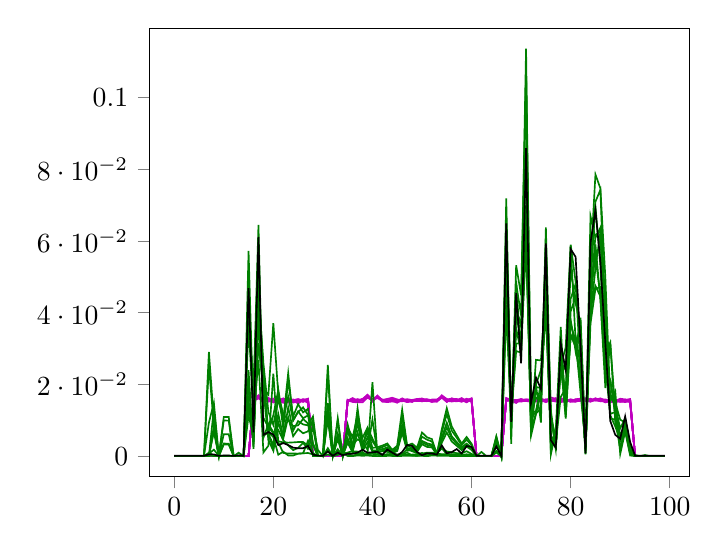
\begin{tikzpicture}

\definecolor{color0}{rgb}{0.75,0,0.75}

\begin{axis}[
xmin=-4.95, xmax=103.95,
ymin=-0.00568306442848251, ymax=0.119344352998133,
tick align=outside,
tick pos=left,
x grid style={lightgray!92.02614379084967!black},
y grid style={lightgray!92.02614379084967!black}
]
\addplot [semithick, color0, forget plot]
table {%
0 0
1 0
2 0
3 0
4 0
5 0
6 0
7 0
8 0
9 0
10 0
11 0
12 0
13 0
14 0
15 1.68381350081665e-05
16 0.0157604943676438
17 0.0164129720992103
18 0.0153647981949519
19 0.0155879034838101
20 0.0160509521965347
21 0.0150911785010692
22 0.0157647039013959
23 0.0150953880348213
24 0.0154952937412652
25 0.0158278469076765
26 0.0155415986125377
27 0.0160383235952786
28 0
29 0
30 0
31 0
32 0
33 0
34 0
35 0.0155836939500581
36 0.0151206452373335
37 0.0149901496910202
38 0.0149901496910202
39 0.016379295829194
40 0.0159120375827173
41 0.0163666672279378
42 0.0152890265874152
43 0.0155163414100254
44 0.015571065348802
45 0.0154363602687366
46 0.0156468369563387
47 0.0155921130175622
48 0.0157099799626193
49 0.0153984744649683
50 0.0160214854602704
51 0.0153311219249356
52 0.0157941706376602
53 0.0158278469076765
54 0.0164424388354746
55 0.0154616174712489
56 0.015571065348802
57 0.0158615231776928
58 0.0154658270050009
59 0.0154826651400091
60 0.015373217262456
61 0
62 0
63 0
64 0
65 0
66 0
67 0.0157141894963714
68 0.0154531984037448
69 0.0154405698024887
70 0.0157183990301234
71 0.0156847227601071
72 0.0155963225513142
73 0.0156005320850663
74 0.0155879034838101
75 0.015579484416306
76 0.0154111030662244
77 0.015571065348802
78 0.016181447742848
79 0.0157436562326357
80 0.0153058647224233
81 0.0151753691761101
82 0.015680513226355
83 0.0154237316674805
84 0.0154321507349846
85 0.0157352371651316
86 0.0161225142703194
87 0.0155205509437775
88 0.015474246072505
89 0.0155626462812979
90 0.0155163414100254
91 0.0156426274225867
92 0.0159415043189816
93 0
94 0
95 0
96 0
97 0
98 0
99 0
};
\addplot [semithick, color0, forget plot]
table {%
0 0
1 0
2 0
3 0
4 0
5 0
6 0
7 0
8 0
9 0
10 0
11 0
12 0
13 0
14 0
15 0
16 0.0158067226890756
17 0.0162100840336134
18 0.0159747899159664
19 0.0156890756302521
20 0.0154285714285714
21 0.0155420168067227
22 0.016
23 0.0149747899159664
24 0.0157605042016807
25 0.0151134453781513
26 0.015718487394958
27 0.0151260504201681
28 0
29 0
30 0
31 0
32 0
33 0
34 0
35 0.0154075630252101
36 0.0157142857142857
37 0.0153529411764706
38 0.015672268907563
39 0.0168949579831933
40 0.0155672268907563
41 0.016672268907563
42 0.0152394957983193
43 0.0153739495798319
44 0.0156638655462185
45 0.0157605042016807
46 0.0153193277310924
47 0.015609243697479
48 0.0156302521008403
49 0.0158865546218487
50 0.015563025210084
51 0.0157899159663866
52 0.015390756302521
53 0.0155714285714286
54 0.016672268907563
55 0.0151638655462185
56 0.0161680672268908
57 0.0156302521008403
58 0.0154873949579832
59 0.0153235294117647
60 0.0157268907563025
61 0
62 0
63 0
64 0
65 0
66 0
67 0.0155252100840336
68 0.0157058823529412
69 0.0156302521008403
70 0.0154285714285714
71 0.0156974789915966
72 0.0158109243697479
73 0.0157983193277311
74 0.0150882352941176
75 0.0158739495798319
76 0.0155588235294118
77 0.0156218487394958
78 0.0152310924369748
79 0.0154201680672269
80 0.0154789915966387
81 0.0157983193277311
82 0.0157310924369748
83 0.0156554621848739
84 0.0152857142857143
85 0.0158235294117647
86 0.0153403361344538
87 0.0152647058823529
88 0.0152731092436975
89 0.0155
90 0.0155168067226891
91 0.0155756302521008
92 0.0157689075630252
93 0
94 0
95 0
96 0
97 0
98 0
99 0
};
\addplot [semithick, color0, forget plot]
table {%
0 0
1 0
2 0
3 0
4 0
5 0
6 0
7 0
8 0
9 0
10 0
11 0
12 0
13 0
14 0
15 0
16 0.0154243697478992
17 0.0168949579831933
18 0.0155882352941176
19 0.0155
20 0.0156470588235294
21 0.0154957983193277
22 0.0161134453781513
23 0.0155252100840336
24 0.0153403361344538
25 0.0156764705882353
26 0.0158025210084034
27 0.0156974789915966
28 0
29 0
30 0
31 0
32 0
33 0
34 0
35 0.0154789915966387
36 0.0162100840336134
37 0.0154453781512605
38 0.0156008403361345
39 0.0166848739495798
40 0.0152352941176471
41 0.0168865546218487
42 0.0153571428571429
43 0.0152352941176471
44 0.0158151260504202
45 0.0152352941176471
46 0.0153235294117647
47 0.0156806722689076
48 0.0155294117647059
49 0.0154495798319328
50 0.0159663865546218
51 0.0155546218487395
52 0.0151134453781513
53 0.015453781512605
54 0.016453781512605
55 0.0155336134453782
56 0.0154915966386555
57 0.0154873949579832
58 0.015718487394958
59 0.0152310924369748
60 0.0156638655462185
61 0
62 0
63 0
64 0
65 0
66 0
67 0.0155168067226891
68 0.0158403361344538
69 0.0155924369747899
70 0.0159411764705882
71 0.0154789915966387
72 0.015390756302521
73 0.0155210084033613
74 0.0160336134453781
75 0.0154411764705882
76 0.0155840336134454
77 0.0159579831932773
78 0.0150588235294118
79 0.0154579831932773
80 0.0158109243697479
81 0.0154621848739496
82 0.0155588235294118
83 0.0153109243697479
84 0.0154243697478992
85 0.016063025210084
86 0.0156554621848739
87 0.0155210084033613
88 0.0154663865546218
89 0.0155378151260504
90 0.0153529411764706
91 0.0150756302521008
92 0.0154033613445378
93 0
94 0
95 0
96 0
97 0
98 0
99 0
};
\addplot [semithick, color0, forget plot]
table {%
0 0
1 0
2 0
3 0
4 0
5 0
6 0
7 0
8 0
9 0
10 0
11 0
12 0
13 0
14 0
15 0
16 0.0154243697478992
17 0.0161260504201681
18 0.0162436974789916
19 0.0155294117647059
20 0.0150168067226891
21 0.0157605042016807
22 0.0156470588235294
23 0.0159873949579832
24 0.0154663865546218
25 0.0154411764705882
26 0.015844537815126
27 0.0156302521008403
28 0
29 0
30 0
31 0
32 0
33 0
34 0
35 0.0153613445378151
36 0.0156932773109244
37 0.0152478991596639
38 0.0156806722689076
39 0.0170504201680672
40 0.0158403361344538
41 0.0165840336134454
42 0.0157521008403361
43 0.0155084033613445
44 0.0156386554621849
45 0.0157268907563025
46 0.0156386554621849
47 0.0156596638655462
48 0.0150924369747899
49 0.015936974789916
50 0.0160798319327731
51 0.015546218487395
52 0.0152731092436975
53 0.0156134453781513
54 0.016672268907563
55 0.0153151260504202
56 0.0154033613445378
57 0.0153067226890756
58 0.0155
59 0.0157310924369748
60 0.015844537815126
61 0
62 0
63 0
64 0
65 0
66 0
67 0.0156974789915966
68 0.0155714285714286
69 0.015218487394958
70 0.0153949579831933
71 0.0153613445378151
72 0.0152352941176471
73 0.0157016806722689
74 0.0157773109243697
75 0.0150378151260504
76 0.0157268907563025
77 0.0161806722689076
78 0.0157268907563025
79 0.0155966386554622
80 0.0152226890756303
81 0.0152689075630252
82 0.0154831932773109
83 0.0154327731092437
84 0.0159033613445378
85 0.015546218487395
86 0.0156386554621849
87 0.0149873949579832
88 0.0153235294117647
89 0.0151428571428571
90 0.0160252100840336
91 0.0158193277310924
92 0.0151638655462185
93 0
94 0
95 0
96 0
97 0
98 0
99 0
};
\addplot [semithick, color0, forget plot]
table {%
0 0
1 0
2 0
3 0
4 0
5 0
6 0
7 0
8 0
9 0
10 0
11 0
12 0
13 0
14 0
15 0
16 0.0157436974789916
17 0.0168193277310924
18 0.0155336134453782
19 0.0154873949579832
20 0.0158529411764706
21 0.0156932773109244
22 0.0148655462184874
23 0.0150798319327731
24 0.0153613445378151
25 0.015563025210084
26 0.0155756302521008
27 0.0148655462184874
28 0
29 0
30 0
31 0
32 0
33 0
34 0
35 0.0154705882352941
36 0.015936974789916
37 0.0155126050420168
38 0.0154579831932773
39 0.0169411764705882
40 0.0157142857142857
41 0.0161932773109244
42 0.015718487394958
43 0.0152941176470588
44 0.0160378151260504
45 0.0153403361344538
46 0.0156008403361345
47 0.015890756302521
48 0.0156218487394958
49 0.0156134453781513
50 0.0155798319327731
51 0.0157394957983193
52 0.015172268907563
53 0.015453781512605
54 0.0167352941176471
55 0.0158571428571429
56 0.0159957983193277
57 0.0155336134453782
58 0.015172268907563
59 0.015718487394958
60 0.0158655462184874
61 0
62 0
63 0
64 0
65 0
66 0
67 0.0157689075630252
68 0.0157857142857143
69 0.0155588235294118
70 0.0156638655462185
71 0.0158487394957983
72 0.0156932773109244
73 0.0154243697478992
74 0.0157310924369748
75 0.0155504201680672
76 0.0157773109243697
77 0.0155126050420168
78 0.0152100840336134
79 0.0154705882352941
80 0.0154957983193277
81 0.0156848739495798
82 0.015936974789916
83 0.015453781512605
84 0.0151806722689076
85 0.0157310924369748
86 0.0153067226890756
87 0.0156302521008403
88 0.0151008403361345
89 0.0153319327731092
90 0.0153067226890756
91 0.0156008403361345
92 0.0156344537815126
93 0
94 0
95 0
96 0
97 0
98 0
99 0
};
\addplot [semithick, color0, forget plot]
table {%
0 0
1 0
2 0
3 0
4 0
5 0
6 0
7 0
8 0
9 0
10 0
11 0
12 0
13 0
14 0
15 0
16 0.0153319327731092
17 0.0165420168067227
18 0.0154285714285714
19 0.0151974789915966
20 0.0156470588235294
21 0.0156218487394958
22 0.0153151260504202
23 0.0153025210084034
24 0.0150294117647059
25 0.0156302521008403
26 0.0151134453781513
27 0.0157899159663866
28 0
29 0
30 0
31 0
32 0
33 0
34 0
35 0.0156470588235294
36 0.0155294117647059
37 0.0159201680672269
38 0.0155
39 0.0163571428571429
40 0.0155546218487395
41 0.016546218487395
42 0.0156638655462185
43 0.0155294117647059
44 0.0158109243697479
45 0.0153655462184874
46 0.0161176470588235
47 0.0154873949579832
48 0.0155
49 0.0154789915966387
50 0.0154957983193277
51 0.0157647058823529
52 0.0153403361344538
53 0.0151554621848739
54 0.0163991596638655
55 0.0157689075630252
56 0.0155966386554622
57 0.0155924369747899
58 0.0153781512605042
59 0.0160252100840336
60 0.0154411764705882
61 0
62 0
63 0
64 0
65 0
66 0
67 0.0162142857142857
68 0.0156890756302521
69 0.0151764705882353
70 0.0157857142857143
71 0.015390756302521
72 0.0158865546218487
73 0.015672268907563
74 0.0158613445378151
75 0.0157142857142857
76 0.0157857142857143
77 0.0154579831932773
78 0.0156680672268908
79 0.0155546218487395
80 0.0152268907563025
81 0.0156806722689076
82 0.0154789915966387
83 0.0158067226890756
84 0.0153445378151261
85 0.0157058823529412
86 0.0158613445378151
87 0.0153991596638655
88 0.0156554621848739
89 0.0158403361344538
90 0.0151974789915966
91 0.0155042016806723
92 0.0155252100840336
93 0
94 0
95 0
96 0
97 0
98 0
99 0
};
\addplot [semithick, color0, forget plot]
table {%
0 0
1 0
2 0
3 0
4 0
5 0
6 0
7 0
8 0
9 0
10 0
11 0
12 0
13 0
14 0
15 0
16 0.0155672268907563
17 0.0162142857142857
18 0.0150672268907563
19 0.0156470588235294
20 0.0152563025210084
21 0.0149201680672269
22 0.0155210084033613
23 0.0161344537815126
24 0.0156134453781513
25 0.0159327731092437
26 0.0153193277310924
27 0.0157268907563025
28 0
29 0
30 0
31 0
32 0
33 0
34 0
35 0.0156806722689076
36 0.0153235294117647
37 0.0153445378151261
38 0.0159159663865546
39 0.0162899159663866
40 0.0157016806722689
41 0.0166890756302521
42 0.0156848739495798
43 0.0159663865546218
44 0.0163025210084034
45 0.0158025210084034
46 0.0155168067226891
47 0.0150756302521008
48 0.0152689075630252
49 0.0157521008403361
50 0.0152689075630252
51 0.0156932773109244
52 0.0154243697478992
53 0.0153781512605042
54 0.0162773109243697
55 0.0151176470588235
56 0.0158823529411765
57 0.015953781512605
58 0.0153445378151261
59 0.0157226890756303
60 0.0157394957983193
61 0
62 0
63 0
64 0
65 0
66 0
67 0.0160798319327731
68 0.0156386554621849
69 0.0155042016806723
70 0.0152016806722689
71 0.0155420168067227
72 0.0157689075630252
73 0.0154915966386555
74 0.015436974789916
75 0.015172268907563
76 0.0155588235294118
77 0.0161134453781513
78 0.0154579831932773
79 0.0153739495798319
80 0.0153151260504202
81 0.0158739495798319
82 0.0160336134453781
83 0.0153361344537815
84 0.0160378151260504
85 0.0154831932773109
86 0.0155420168067227
87 0.0158403361344538
88 0.0153571428571429
89 0.0158193277310924
90 0.0151554621848739
91 0.0152478991596639
92 0.0155798319327731
93 0
94 0
95 0
96 0
97 0
98 0
99 0
};
\addplot [semithick, color0, forget plot]
table {%
0 0
1 0
2 0
3 0
4 0
5 0
6 0
7 0
8 0
9 0
10 0
11 0
12 0
13 0
14 0
15 0
16 0.0160714285714286
17 0.0169789915966387
18 0.0155588235294118
19 0.0154453781512605
20 0.0149873949579832
21 0.0156680672268908
22 0.0156680672268908
23 0.0155126050420168
24 0.0157983193277311
25 0.015281512605042
26 0.0158193277310924
27 0.0152983193277311
28 0
29 0
30 0
31 0
32 0
33 0
34 0
35 0.0157268907563025
36 0.0153655462184874
37 0.015546218487395
38 0.0159663865546218
39 0.0166008403361345
40 0.0154201680672269
41 0.0167563025210084
42 0.0155210084033613
43 0.0155126050420168
44 0.015609243697479
45 0.0153865546218487
46 0.0155756302521008
47 0.015563025210084
48 0.0153865546218487
49 0.0157941176470588
50 0.0158193277310924
51 0.0158697478991597
52 0.0156008403361345
53 0.0156680672268908
54 0.0166218487394958
55 0.0154159663865546
56 0.0152563025210084
57 0.0154201680672269
58 0.0153235294117647
59 0.0156344537815126
60 0.0159327731092437
61 0
62 0
63 0
64 0
65 0
66 0
67 0.015453781512605
68 0.0154579831932773
69 0.0148235294117647
70 0.0158529411764706
71 0.0155294117647059
72 0.0151176470588235
73 0.0160084033613445
74 0.0153781512605042
75 0.0155672268907563
76 0.0163865546218487
77 0.015936974789916
78 0.0153025210084034
79 0.0155378151260504
80 0.0152605042016807
81 0.015436974789916
82 0.0154747899159664
83 0.0153739495798319
84 0.0153571428571429
85 0.0157521008403361
86 0.0159705882352941
87 0.0156554621848739
88 0.0150420168067227
89 0.0155252100840336
90 0.0159075630252101
91 0.015436974789916
92 0.0150714285714286
93 0
94 0
95 0
96 0
97 0
98 0
99 0
};
\addplot [semithick, color0, forget plot]
table {%
0 0
1 0
2 0
3 0
4 0
5 0
6 0
7 0
8 0
9 0
10 0
11 0
12 0
13 0
14 0
15 0
16 0.015827731092437
17 0.0167268907563025
18 0.0155924369747899
19 0.0162521008403361
20 0.0155420168067227
21 0.0155546218487395
22 0.0157857142857143
23 0.0155924369747899
24 0.0149495798319328
25 0.0152731092436975
26 0.0153697478991597
27 0.0154957983193277
28 0
29 0
30 0
31 0
32 0
33 0
34 0
35 0.0154957983193277
36 0.0155840336134454
37 0.0152857142857143
38 0.0156596638655462
39 0.0167773109243697
40 0.015546218487395
41 0.0164201680672269
42 0.0156302521008403
43 0.0154957983193277
44 0.0153865546218487
45 0.0149033613445378
46 0.0157857142857143
47 0.0151344537815126
48 0.0156344537815126
49 0.0153655462184874
50 0.0153697478991597
51 0.0153739495798319
52 0.0155210084033613
53 0.0154663865546218
54 0.0169789915966387
55 0.015936974789916
56 0.0152899159663866
57 0.0155966386554622
58 0.0162016806722689
59 0.0154495798319328
60 0.016172268907563
61 0
62 0
63 0
64 0
65 0
66 0
67 0.0158403361344538
68 0.015844537815126
69 0.0152478991596639
70 0.0153655462184874
71 0.0157983193277311
72 0.015546218487395
73 0.0158697478991597
74 0.0156176470588235
75 0.0156512605042017
76 0.0155378151260504
77 0.0152142857142857
78 0.0155672268907563
79 0.0157647058823529
80 0.0152773109243697
81 0.0156176470588235
82 0.0155042016806723
83 0.0156764705882353
84 0.0154915966386555
85 0.0161344537815126
86 0.0155714285714286
87 0.0156806722689076
88 0.0152731092436975
89 0.0154789915966387
90 0.0153865546218487
91 0.0154873949579832
92 0.0151302521008403
93 0
94 0
95 0
96 0
97 0
98 0
99 0
};
\addplot [semithick, color0, forget plot]
table {%
0 0
1 0
2 0
3 0
4 0
5 0
6 0
7 0
8 0
9 0
10 0
11 0
12 0
13 0
14 0
15 0
16 0.0156974789915966
17 0.0165798319327731
18 0.0149621848739496
19 0.0161176470588235
20 0.0154033613445378
21 0.0157899159663866
22 0.0158235294117647
23 0.0154453781512605
24 0.0155840336134454
25 0.0146470588235294
26 0.0156974789915966
27 0.0158655462184874
28 0
29 0
30 0
31 0
32 0
33 0
34 0
35 0.0154117647058824
36 0.0154663865546218
37 0.0152983193277311
38 0.0159243697478992
39 0.0171386554621849
40 0.0153571428571429
41 0.0168067226890756
42 0.0152436974789916
43 0.0150756302521008
44 0.0152521008403361
45 0.0152941176470588
46 0.0153781512605042
47 0.0157563025210084
48 0.0156806722689076
49 0.0158949579831933
50 0.0158991596638655
51 0.0155
52 0.0154831932773109
53 0.0154621848739496
54 0.0165966386554622
55 0.0155882352941176
56 0.0155252100840336
57 0.0156008403361345
58 0.0156470588235294
59 0.0150042016806723
60 0.0158571428571429
61 0
62 0
63 0
64 0
65 0
66 0
67 0.0154747899159664
68 0.0158697478991597
69 0.0152478991596639
70 0.0155672268907563
71 0.015453781512605
72 0.0157436974789916
73 0.0152310924369748
74 0.0156470588235294
75 0.0154621848739496
76 0.0154579831932773
77 0.015953781512605
78 0.0157478991596639
79 0.0154285714285714
80 0.0158319327731092
81 0.0155588235294118
82 0.0156134453781513
83 0.0161890756302521
84 0.0157899159663866
85 0.0155756302521008
86 0.0155210084033613
87 0.0154159663865546
88 0.0155798319327731
89 0.0150840336134454
90 0.015281512605042
91 0.0157899159663866
92 0.0157268907563025
93 0
94 0
95 0
96 0
97 0
98 0
99 0
};
\addplot [semithick, green!50.0!black, forget plot]
table {%
0 0
1 0
2 0
3 0
4 0
5 0
6 0
7 0.0290635894185418
8 0.00989914431125445
9 0
10 0
11 0
12 0
13 0.000223709475960553
14 0
15 0.0475569060979475
16 0.0102347085251953
17 0.0314498238287877
18 0.0186610987863761
19 0.0171510598236424
20 0.0371171305531217
21 0.0171697022799724
22 0.0118193173132492
23 0.0100669264182249
24 0.00838910534852072
25 0.00859417236815123
26 0.0103652057195056
27 0.00913480360172256
28 5.59273689901381e-05
29 0
30 0
31 0.0115769653809586
32 0
33 0.00195745791465484
34 1.8642456330046e-05
35 0.00883652430044183
36 0.00320650248876792
37 0.00467925653884156
38 0.00397084319829981
39 0.00182696072034451
40 0.0101974236125352
41 0.00109990492347272
42 0.00136089931209336
43 0.00119311720512295
44 0.000782983165861934
45 0.000260994388620645
46 0.000559273689901381
47 0.00199474282731493
48 0.00136089931209336
49 0.000876195447512164
50 0.000689770884211704
51 0.000988050185492441
52 0.000969407729162394
53 0.000857552991182118
54 0.0021438824779553
55 0.00130497194310322
56 0.00108126246714267
57 0.000838910534852072
58 0.000782983165861934
59 0.00137954176842341
60 0.000633843515221566
61 1.8642456330046e-05
62 0
63 1.8642456330046e-05
64 0
65 0.00357935161536884
66 0
67 0.0512108275386365
68 0.0115023955556384
69 0.0356630189593781
70 0.0288212374862512
71 0.059898212188438
72 0.011315970992338
73 0.0163307917451203
74 0.0153427415596279
75 0.0462332916985142
76 0.00568594918066404
77 0.00361663652802893
78 0.0165172163084208
79 0.0189407356313268
80 0.0438843422009284
81 0.0480788948751888
82 0.0241979083163998
83 0.000503346320911243
84 0.0390186610987864
85 0.0524039447437594
86 0.0625454409873045
87 0.0251673160455622
88 0.0114278257303182
89 0.00827725061054044
90 0.0046978989951716
91 0.00932122816502302
92 0.00139818422475345
93 0
94 0
95 0
96 0
97 0
98 0
99 0
};
\addplot [semithick, green!50.0!black, forget plot]
table {%
0 0
1 0
2 0
3 0
4 0
5 0
6 0
7 0.000973199580775565
8 0.000199630683236013
9 2.49538354045017e-05
10 2.49538354045017e-05
11 2.49538354045017e-05
12 0
13 0.000973199580775565
14 2.49538354045017e-05
15 0.0572191445825223
16 0.0106802415531267
17 0.0526026850326895
18 0.0106552877177222
19 0.00810999650646304
20 0.00641313569895693
21 0.00731147377351899
22 0.0044417827020013
23 0.0029944602485402
24 0.00167190697210161
25 0.00229575285721415
26 0.00369316763986625
27 0.00202126066776464
28 0.00324399860258522
29 0
30 0
31 0.0014972301242701
32 0
33 0.00127264560562959
34 0.000573938214303538
35 0.00102310725158457
36 0.00137246094724759
37 0.00127264560562959
38 0.00104806108698907
39 0.000374307531067525
40 0.000773568897539552
41 0.000973199580775565
42 0.00029944602485402
43 0.00029944602485402
44 0.000923291909966562
45 0.000399261366472027
46 0.000548984378899037
47 0.000998153416180067
48 0.000224584518640515
49 0.000199630683236013
50 0.000923291909966562
51 0.000174676847831512
52 0.00089833807456206
53 0.000948245745371063
54 0.000349353695663023
55 0.000424215201876528
56 0.00029944602485402
57 0.00044916903728103
58 0.000324399860258522
59 0.00014972301242701
60 0.00014972301242701
61 0
62 0
63 0
64 0
65 0.000998153416180067
66 0
67 0.0669261865548735
68 0.0111543644258122
69 0.0410740130758098
70 0.0361081998303139
71 0.0837700254529121
72 0.00993162649099166
73 0.0192643609322753
74 0.0190397764136348
75 0.0573439137595448
76 0.00204621450316914
77 0.00459150571442831
78 0.0260767579977042
79 0.0240305434945351
80 0.058990866896242
81 0.0486849328741828
82 0.0320656784947847
83 0.00074861506213505
84 0.0471128412436992
85 0.0709687078904028
86 0.074262614163797
87 0.0373808454359435
88 0.0105055647052952
89 0.0102061186804412
90 0.00184658381993312
91 0.00848430403753057
92 0.000973199580775565
93 0.000324399860258522
94 0
95 0.000324399860258522
96 0
97 0
98 0
99 0
};
\addplot [semithick, green!50.0!black, forget plot]
table {%
0 0
1 0
2 0
3 0
4 0
5 0
6 0
7 0.0249671484888305
8 0.00864513451829311
9 0
10 0
11 0
12 0
13 7.9041229881537e-05
14 9.88015373519212e-06
15 0.0367640520486499
16 0.011263375258119
17 0.0267850967761058
18 0.00103741614219517
19 0.00291464535188168
20 0.0230306383567328
21 0.00385325995672493
22 0.000908974143637675
23 0.000721251222669025
24 0.000741011530139409
25 0.000711371068933833
26 0.000810172606285754
27 0.000879333682432099
28 0.00051376799422999
29 9.88015373519212e-06
30 0
31 0.0102457194233942
32 0
33 0.00159070475136593
34 0.000405086303142877
35 0.00378409888057858
36 0.0010077756809896
37 0.000573048916641143
38 0.00051376799422999
39 0.000523648147965182
40 0.0206297609990811
41 0.00046436722555403
42 0.00046436722555403
43 0.000444606918083645
44 0.000563168762905951
45 0.000494007686759606
46 0.000523648147965182
47 0.000405086303142877
48 0.000444606918083645
49 0.000543408455435567
50 0.000484127533024414
51 0.00065209014652268
52 0.000523648147965182
53 0.000543408455435567
54 0.00051376799422999
55 0.000523648147965182
56 0.000582929070376335
57 0.000444606918083645
58 0.000345805380731724
59 0.000523648147965182
60 0.000365565688202108
61 0
62 0
63 0
64 0
65 0.00442630887336607
66 0
67 0.0554177823006926
68 0.00345805380731724
69 0.0481953899202672
70 0.0392538507899183
71 0.11366128856965
72 0.00723227253416063
73 0.0268641380059874
74 0.0267060555462243
75 0.0465058836315493
76 0.00157094444389555
77 0.00697538853704564
78 0.0360329206722457
79 0.0109966111072688
80 0.03805835218796
81 0.0292057344412279
82 0.0385918804896604
83 0.00346793396105243
84 0.0669874423246026
85 0.060940788238665
86 0.0637467518994596
87 0.0436011184334028
88 0.011777143252349
89 0.0123106715540494
90 0.00223291474415342
91 0.00735083437898294
92 0.000661970300257872
93 0
94 0
95 0
96 0
97 0
98 0
99 0
};
\addplot [semithick, green!50.0!black, forget plot]
table {%
0 0
1 0
2 0
3 0
4 0
5 0
6 0
7 0.000111823468018488
8 5.59117340092441e-05
9 0
10 3.72744893394961e-05
11 3.72744893394961e-05
12 0
13 0
14 0
15 0.0421201729536305
16 0.016493961532727
17 0.0591918890711197
18 0.00568435962427315
19 0.0065975846130908
20 0.00536752646488743
21 0.000410019382734457
22 0.00124869539287312
23 0.000205009691367228
24 0.00018637244669748
25 0.000689578052780677
26 0.000801401520799165
27 0.00428656627404205
28 0.000894587744147905
29 0
30 0
31 0.000484568361413449
32 0
33 0.000428656627404205
34 0.000838676010138661
35 5.59117340092441e-05
36 1.8637244669748e-05
37 0.00018637244669748
38 0.000111823468018488
39 0.000167735202027732
40 5.59117340092441e-05
41 1.8637244669748e-05
42 0
43 7.45489786789921e-05
44 7.45489786789921e-05
45 0
46 7.45489786789921e-05
47 9.31862233487401e-05
48 7.45489786789921e-05
49 7.45489786789921e-05
50 9.31862233487401e-05
51 0
52 0.00018637244669748
53 0.000149097957357984
54 7.45489786789921e-05
55 0.000130460712688236
56 1.8637244669748e-05
57 1.8637244669748e-05
58 1.8637244669748e-05
59 1.8637244669748e-05
60 0
61 0
62 0
63 0
64 0
65 0.00149097957357984
66 0
67 0.0603473982406441
68 0.00808856418667064
69 0.0532279707768004
70 0.0448784851647532
71 0.106344118085582
72 0.00629938869837483
73 0.0198859400626211
74 0.00935589682421351
75 0.0608878783360668
76 0.000428656627404205
77 0.00708215297450425
78 0.0269867302817951
79 0.0161584911286715
80 0.0523333830326525
81 0.0425115550916952
82 0.0371813031161473
83 0.000913224988817653
84 0.0534329804681676
85 0.0785559862829879
86 0.0746794393916803
87 0.0498359922469062
88 0.0153570896078724
89 0.0181154018189951
90 0.000596391829431937
91 0.00687714328313702
92 0.00018637244669748
93 0
94 0
95 0
96 0
97 0
98 0
99 0
};
\addplot [semithick, green!50.0!black, forget plot]
table {%
0 0
1 0
2 0
3 0
4 0
5 0
6 0
7 0.000722519622976124
8 0.00180629905744031
9 0.000131367204177477
10 0.000131367204177477
11 0.000131367204177477
12 0
13 6.56836020887385e-05
14 0
15 0.0412821439127722
16 0.0183585667838024
17 0.0644684554500969
18 0.00515616276396598
19 0.00896581168511281
20 0.00669972741305133
21 0.0041709087326349
22 0.0038424907221912
23 0.00377680712010247
24 0.0038424907221912
25 0.00394101612532431
26 0.00394101612532431
27 0.0029886038950376
28 0.00817760846004795
29 0.000164209005221846
30 0
31 0.00223324247101711
32 0
33 0.000394101612532431
34 0.00101809583237545
35 0.000722519622976124
36 9.85254031331078e-05
37 0.000591152418798647
38 0.000689677821931755
39 0.000722519622976124
40 0.000656836020887386
41 0.000394101612532431
42 0.000131367204177477
43 0.000558310617754278
44 6.56836020887385e-05
45 0.000131367204177477
46 0.000361259811488062
47 0.000361259811488062
48 0.000197050806266216
49 9.85254031331078e-05
50 0.000295576209399323
51 6.56836020887385e-05
52 0.000361259811488062
53 0.000821045026109232
54 0.00223324247101711
55 0.000525468816709908
56 6.56836020887385e-05
57 9.85254031331078e-05
58 0
59 0
60 3.28418010443693e-05
61 0
62 0.00118230483759729
63 0
64 0
65 0.00476206115143354
66 0
67 0.07185786068508
68 0.00926138789451214
69 0.0489671253571546
70 0.026766067851161
71 0.106703011593156
72 0.017077736543072
73 0.017701730762915
74 0.0160267989096522
75 0.0507734244145949
76 0.010936319747775
77 0.00525468816709908
78 0.0251239777989425
79 0.0303786659660416
80 0.058786823869421
81 0.0320864396203488
82 0.0175375217576932
83 0.00351407271174751
84 0.0512332096292161
85 0.0697888272192847
86 0.0530723504877007
87 0.0244014581759664
88 0.02134717067884
89 0.011297579559263
90 0.00574731518276462
91 0.00870307727675786
92 0.00302144569608197
93 0
94 0
95 0
96 0
97 0
98 0
99 0
};
\addplot [semithick, green!50.0!black, forget plot]
table {%
0 0
1 0
2 0
3 0
4 0
5 0
6 0
7 0
8 0.00754084625052367
9 0
10 0.00612111902434483
11 0.00612111902434483
12 0
13 0
14 0
15 0.0209002467066983
16 0.00258343806730904
17 0.0456174649723037
18 0.0258809291067356
19 0.0123353349159801
20 0.00870455709165387
21 0.0158264674393707
22 0.0102173811851231
23 0.0166410650281618
24 0.00996136480007448
25 0.0123120606991575
26 0.0136154168412233
27 0.0114741888935437
28 0.00823907275520179
29 0.00174556626169529
30 0
31 0.0148489503328213
32 0
33 0.00556253782060234
34 9.30968672904157e-05
35 0.00807615323744356
36 0.00523669878508588
37 0.0114043662430759
38 0.00514360191779547
39 0.00791323371968533
40 0.00491085974956943
41 0.00216450216450216
42 0.0017921146953405
43 0.00221105059814737
44 0.00109388819066238
45 0.00172229204487269
46 0.00768049155145929
47 0.00188521156263092
48 0.00214122794767956
49 0.00148954987664665
50 0.00384024577572965
51 0.00314201927105153
52 0.00279290601871247
53 0.000581855420565098
54 0.00458502071405297
55 0.00802960480379835
56 0.00495740818321464
57 0.00349113252339059
58 0.00211795373085696
59 0.00314201927105153
60 0.00207140529721175
61 0
62 0
63 0
64 0
65 0.0035376809570358
66 0
67 0.055765023506959
68 0.011637108411302
69 0.0347018572825024
70 0.0312339989759345
71 0.0699622957687474
72 0.00567890890471536
73 0.0117302052785924
74 0.0178513243029372
75 0.0439649955778988
76 0.0116603826281246
77 0.00202485686356654
78 0.0262998650095424
79 0.0104733975701718
80 0.0339570823441791
81 0.0309314341572406
82 0.0213191826095052
83 0.00148954987664665
84 0.0459665782246427
85 0.0556253782060234
86 0.0445468509984639
87 0.0219941348973607
88 0.0211329888749244
89 0.0126611739514965
90 0.00500395661685984
91 0.00726155564865242
92 0.00148954987664665
93 6.98226504678118e-05
94 0
95 6.98226504678118e-05
96 0
97 0
98 0
99 0
};
\addplot [semithick, green!50.0!black, forget plot]
table {%
0 0
1 0
2 0
3 0
4 0
5 0
6 0
7 7.32421875e-05
8 0.0132080078125
9 0
10 0.0032958984375
11 0.0031982421875
12 0
13 0
14 0
15 0.014501953125
16 0.0041015625
17 0.0371826171875
18 0.01962890625
19 0.00634765625
20 0.001904296875
21 0.0181884765625
22 0.007666015625
23 0.021044921875
24 0.011083984375
25 0.014501953125
26 0.01220703125
27 0.0132080078125
28 0.0032958984375
29 0
30 0
31 0.02314453125
32 0
33 0.0099365234375
34 0
35 0.0078125
36 0.0024658203125
37 0.01337890625
38 0.0029541015625
39 0.0077392578125
40 0.002294921875
41 0.0025146484375
42 0.0029541015625
43 0.0035400390625
44 0.0017578125
45 0.0029052734375
46 0.01298828125
47 0.0029541015625
48 0.003515625
49 0.0023681640625
50 0.0066162109375
51 0.0052734375
52 0.0047607421875
53 0.0005859375
54 0.0075439453125
55 0.01337890625
56 0.00830078125
57 0.0058349609375
58 0.003515625
59 0.0053466796875
60 0.0034912109375
61 0
62 0
63 0
64 0
65 0.0054931640625
66 0
67 0.042333984375
68 0.0114990234375
69 0.0313720703125
70 0.0316162109375
71 0.06708984375
72 0.00703125
73 0.0199462890625
74 0.0240478515625
75 0.03955078125
76 0.00576171875
77 0.0024658203125
78 0.0301025390625
79 0.01240234375
80 0.033642578125
81 0.0304931640625
82 0.021533203125
83 0.002392578125
84 0.0369384765625
85 0.0466552734375
86 0.0471923828125
87 0.0241455078125
88 0.01708984375
89 0.01396484375
90 0.0077392578125
91 0.0106201171875
92 0.0023681640625
93 0
94 0
95 0
96 0
97 0
98 0
99 0
};
\addplot [semithick, green!50.0!black, forget plot]
table {%
0 0
1 0
2 0
3 0
4 0
5 0
6 0
7 0.00933339231211572
8 0.0148847702039191
9 0
10 0.00351660989958862
11 0.00349449285619498
12 0
13 0
14 0
15 0.0113239262175432
16 0.00563984606537798
17 0.0316716061396912
18 0.0192639447958597
19 0.00687840049542177
20 0.0114123943911178
21 0.018511965320476
22 0.00997478657053125
23 0.0231786614765338
24 0.00997478657053125
25 0.0124961295174061
26 0.0105719467421595
27 0.0113902773477242
28 0.00360507807316318
29 0
30 0
31 0.0254567169460786
32 0
33 0.0105719467421595
34 0
35 0.00723227318972
36 0.00207900207900208
37 0.0117883841288097
38 0.00307426903171584
39 0.00659087893130446
40 0.0041801212013978
41 0.00210111912239572
42 0.0025434599902685
43 0.00309638607510948
44 0.0015260759941611
45 0.00260981112044942
46 0.0110806387402132
47 0.0025434599902685
48 0.00311850311850312
49 0.0020347679922148
50 0.00544079267483523
51 0.00460034502587694
52 0.00409165302782324
53 0.000597160171628257
54 0.00665723006148538
55 0.0118105011722033
56 0.0071216879727518
57 0.00517538815411156
58 0.0030521519883222
59 0.0045782279824833
60 0.00307426903171584
61 0
62 0
63 0
64 0
65 0.00466669615605786
66 0
67 0.0401866678462423
68 0.0110585216968196
69 0.0293050824965719
70 0.0288848586720927
71 0.066129959746981
72 0.0126288317777679
73 0.0123634272570443
74 0.0206794355730526
75 0.040695359844296
76 0.00579466536913345
77 0.00245499181669394
78 0.031870659530234
79 0.0130711726456407
80 0.0372451010748883
81 0.0316494890962976
82 0.0205467333126908
83 0.00238864068651303
84 0.0408501791480515
85 0.0474852921661432
86 0.0445437253947892
87 0.0262971645950369
88 0.0172070597602513
89 0.0149511213341001
90 0.010173839961074
91 0.00937762639890299
92 0.0025434599902685
93 0
94 0
95 0
96 0
97 0
98 0
99 0
};
\addplot [semithick, green!50.0!black, forget plot]
table {%
0 0
1 0
2 0
3 0
4 0
5 0
6 0
7 0.000223490928300047
8 0.00678599727747415
9 0
10 0.00995550498791117
11 0.00989455291655661
12 0
13 0
14 0
15 0.0239541640423414
16 0.00201141835470042
17 0.0435197789471546
18 0.0186106991202584
19 0.00442918385176456
20 0.00150348442674577
21 0.00946788841707471
22 0.00487616570836466
23 0.0108494687011114
24 0.00556695585038298
25 0.00755805684796522
26 0.00637965013511043
27 0.00692821877730145
28 0.00995550498791117
29 0
30 0
31 0.0116012109144842
32 0
33 0.0048152136370101
34 0
35 0.0039415672809281
36 0.00121904142709116
37 0.00664377577764684
38 0.00142221499827302
39 0.00392124992380991
40 0.00127999349844572
41 0.00121904142709116
42 0.00144253235539121
43 0.00180824478351856
44 0.000853328998963815
45 0.00144253235539121
46 0.00648123692070136
47 0.00148316706962758
48 0.00176761006928219
49 0.00117840671285479
50 0.00333204656738252
51 0.00258030435400963
52 0.00243808285418233
53 0.000446981856600093
54 0.00373839370974624
55 0.00660314106341047
56 0.0040837887807554
57 0.00290538206790061
58 0.00170665799792763
59 0.00268189113960056
60 0.00172697535504582
61 0
62 0
63 0
64 0
65 0.00280379528230968
66 0
67 0.0594892216420488
68 0.00822852963286536
69 0.040837887807554
70 0.0367337816696804
71 0.0649139559926045
72 0.00733456591966517
73 0.0119262886283752
74 0.0133281862695301
75 0.0637761839939861
76 0.0112964505577115
77 0.00190983156910949
78 0.0249497145411325
79 0.0129218391271663
80 0.0403502712367175
81 0.0444137426603547
82 0.0347426806720982
83 0.0018895142119913
84 0.0432759706617363
85 0.0615412747109856
86 0.0629634897092586
87 0.0285662041081696
88 0.0317560291757248
89 0.00961010991690201
90 0.00426664499481907
91 0.00770027834779252
92 0.00123935878420935
93 0
94 0
95 0
96 0
97 0
98 0
99 0
};
\addplot [semithick, green!50.0!black, forget plot]
table {%
0 0
1 0
2 0
3 0
4 0
5 0
6 0
7 0
8 0.00838462902449527
9 0
10 0.0109177495757023
11 0.0109177495757023
12 0
13 0
14 0
15 0.0155280289788991
16 0.00440762975910024
17 0.0481039592674215
18 0.0236340147427616
19 0.00620614535045723
20 0.00321706310003293
21 0.0117790105631127
22 0.00549687159611926
23 0.0136281885654938
24 0.00711806874889176
25 0.00977784532765914
26 0.00886592192922461
27 0.00858727866859184
28 0.0110697368087747
29 0
30 0
31 0.0147174304025129
32 0
33 0.00630747017250551
34 0.000151987233072422
35 0.00504090989690199
36 0.0016211971527725
37 0.00929655242292981
38 0.00207715885198977
39 0.00526889074651063
40 0.0016211971527725
41 0.00157053474174836
42 0.00200116523545356
43 0.00243179572915875
44 0.00121589786457938
45 0.00197583402994148
46 0.00873926590166426
47 0.00207715885198977
48 0.00243179572915875
49 0.00159586594726043
50 0.00428097373153988
51 0.00359703118271399
52 0.00321706310003293
53 0.000506624110241406
54 0.00521822833548649
55 0.00934721483395395
56 0.0055475340071434
57 0.00395166805988297
58 0.00243179572915875
59 0.0034957063606657
60 0.00238113331813461
61 0
62 0
63 0
64 0
65 0.00547154039060719
66 0
67 0.0618081414494516
68 0.00967652050561086
69 0.0394153557767814
70 0.0323479494389138
71 0.0588950528155635
72 0.0102338070268764
73 0.0125896091394989
74 0.0178331686804975
75 0.0551460343997771
76 0.0127922587835955
77 0.0025584517567191
78 0.0272310459254756
79 0.0151480608962181
80 0.0334625224814449
81 0.0336398409200294
82 0.0250272310459255
83 0.0018745092078932
84 0.0413658586012108
85 0.059072371254148
86 0.0436456670972972
87 0.0190237353395648
88 0.0314106948349672
89 0.0128175899891076
90 0.00595283329533653
91 0.00802999214732629
92 0.00177318438584492
93 0
94 0
95 0
96 0
97 0
98 0
99 0
};
\addplot [semithick, black, forget plot]
table {%
0 0.0001
1 0.0001
2 0.0001
3 0.0001
4 0.0001
5 0.000101904864523726
6 0.0001
7 0.000501926414506217
8 0.00049049722736386
9 0.0001
10 0.000178099445472772
11 0.000178099445472772
12 0.0001
13 0.000193338361662581
14 0.000107619458094905
15 0.0468606143284294
16 0.00663178045185695
17 0.0611280496111383
18 0.0059136465264122
19 0.00671940421994836
20 0.00603555785593067
21 0.00306777892796533
22 0.00364685774317808
23 0.00310016162486868
24 0.00237631310585274
25 0.00219535097609876
26 0.00222963853752583
27 0.00284110004964192
28 0.000420017239985992
29 0.000162860529282963
30 0.0001
31 0.00132673275327964
32 0.0001
33 0.000983857139008932
34 0.000244769703803187
35 0.000669554492594118
36 0.000677173950689022
37 0.00100100091972247
38 0.00178770996802137
39 0.000953379306629313
40 0.0010905295523376
41 0.00122006033995097
42 0.000374300491416565
43 0.00183533158111452
44 0.000983857139008932
45 0.000155241071188058
46 0.00118386791400018
47 0.0031382589153432
48 0.00287157788202154
49 0.00115910467519174
50 0.000239055110232009
51 0.000795275551160043
52 0.000730510157353354
53 0.00044097074974698
54 0.00299920380511119
55 0.000802895009254948
56 0.00112100738471721
57 0.00197057696229907
58 0.000760987989732973
59 0.00282967086249957
60 0.0025991822551287
61 0.0001
62 0.0001
63 0.0001
64 0.0001
65 0.00272109358464718
66 0.0001
67 0.0648882521809737
68 0.00959955937982229
69 0.0454243464775399
70 0.0258594829543487
71 0.0859084322002917
72 0.0148379368200692
73 0.0219507009516626
74 0.0187219555839468
75 0.059335572094312
76 0.00445833003028542
77 0.0023877422929951
78 0.0314274019572002
79 0.0239603330241937
80 0.0577583442686667
81 0.0555601306082867
82 0.0307930820707994
83 0.00077241717687533
84 0.0594384347785932
85 0.0686008331377159
86 0.0542286303062022
87 0.0314731187057696
88 0.00979576042576608
89 0.00594412435879182
90 0.00485644671574419
91 0.0110872585728524
92 0.00398211389935389
93 0.0001
94 0.000101904864523726
95 0.0001
96 0.0001
97 0.0001
98 0.0001
99 0.0001
};
\end{axis}

\end{tikzpicture}



% This file was created by matplotlib2tikz v0.6.16.
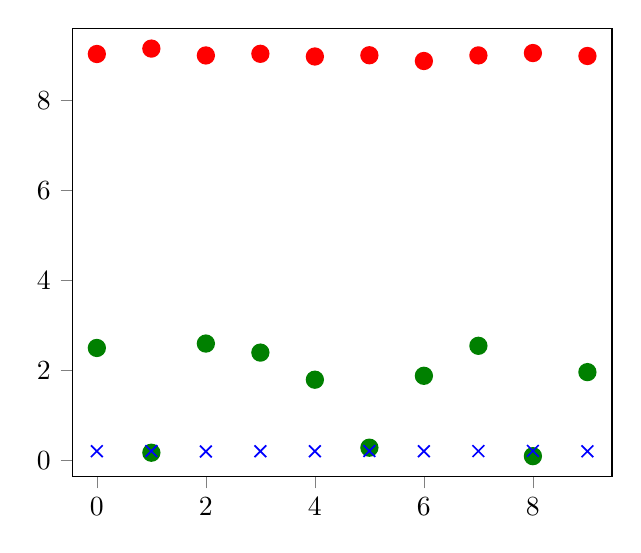
\begin{tikzpicture}

\begin{axis}[
xmin=-0.45, xmax=9.45,
ymin=-0.355007685388461, ymax=9.59965659027902,
tick align=outside,
tick pos=left,
x grid style={lightgray!92.02614379084967!black},
y grid style={lightgray!92.02614379084967!black}
]
\addplot [semithick, red, mark=*, mark size=3, mark options={solid}, only marks, forget plot]
table {%
0 9.02750347531225
1 9.14717185047595
2 8.99510186616441
3 9.03144927124556
4 8.97163566303568
5 8.99947800131077
6 8.8718435448592
7 8.99598152876032
8 9.04840656504152
9 8.98327439481179
};
\addplot [semithick, green!50.0!black, mark=*, mark size=3, mark options={solid}, only marks, forget plot]
table {%
0 2.49976950751913
1 0.173763735912593
2 2.59782384757481
3 2.39709229332274
4 1.79497789921637
5 0.285696898310905
6 1.8819932756703
7 2.54825403343404
8 0.0974770544146064
9 1.96371509633075
};
\addplot [semithick, blue, mark=x, mark size=3, mark options={solid}, only marks, forget plot]
table {%
0 0.207509213272202
1 0.211337361784668
2 0.201447182975852
3 0.206987889158042
4 0.205740484794746
5 0.212382457485257
6 0.206451042994235
7 0.210138553787384
8 0.214205633252259
9 0.205400782735769
};
\end{axis}

\end{tikzpicture}

\section{Implementation}


\pagebreak
\bibliography{thesis}{}
\bibliographystyle{plain}

\end{document}